%% Compressed quadrature-point partial assembly -- formulation and cost model.
%%
%% Build:  make            (pdflatex twice)
%%         make tables     (regenerate tables/ from the cost model)
%%
%% Every derived number in the cost-model sections arrives through \input{tables/...}, written by
%% spikes/inexact_apply_compare/qp/cost_model.py; none is typed in.  Measured results are not yet
%% part of this draft: Section~\ref{sec:plan} states what will be measured.
\documentclass[11pt]{article}

\usepackage[a4paper,margin=1in]{geometry}
\usepackage{amsmath,amssymb}
\usepackage{booktabs}
\usepackage{enumitem}
\usepackage{algorithm}
\usepackage{algpseudocode}
\algrenewcommand\algorithmicrequire{\textbf{Input:}}
\algrenewcommand\algorithmicensure{\textbf{Output:}}
\algnewcommand\Constants{\item[\textbf{Constants:}]}
\usepackage{graphicx}
\usepackage[hidelinks]{hyperref}

\newcommand{\MachineBandwidth}{403}
\newcommand{\MachineNominalBandwidth}{500}
\newcommand{\MachineBandwidthPct}{81}
\newcommand{\MachinePeakFsixtyfour}{3{,}571}
\newcommand{\MachinePeakFthirtytwo}{7{,}142}
\newcommand{\MeasuredDof}{2.74\times10^{6}}
\newcommand{\BsrMeasuredSixtyfour}{575}
\newcommand{\BsrBoundSixtyfour}{574}
\newcommand{\BsrMeasuredThirtytwo}{1{,}029}
\newcommand{\BsrBoundThirtytwo}{1{,}064}
\newcommand{\nqTetFour}{1}
\newcommand{\rTetFour}{1}
\newcommand{\perpointTetFour}{45}
\newcommand{\minimalTetFour}{45}
\newcommand{\storeTetFour}{45}
\newcommand{\flopsTetFour}{192}
\newcommand{\directTetFour}{192}
\newcommand{\rankdiagTetFour}{1}
\newcommand{\rankoffTetFour}{1}
\newcommand{\blocksTetFour}{15}
\newcommand{\bsrsixtyfourTetFour}{383}
\newcommand{\bsrthirtytwoTetFour}{203}
\newcommand{\painteightTetFour}{98}
\newcommand{\pafsixteenTetFour}{188}
\newcommand{\ratiointTetFour}{3.9}
\newcommand{\ratiohalfTetFour}{2.0}
\newcommand{\exactQpPctTetFour}{44}
\newcommand{\exactEaPctTetFour}{62}
\newcommand{\exactBsrPctTetFour}{53}
\newcommand{\nqTetTen}{11}
\newcommand{\rTetTen}{4}
\newcommand{\perpointTetTen}{495}
\newcommand{\minimalTetTen}{450}
\newcommand{\storeTetTen}{450}
\newcommand{\flopsTetTen}{2856}
\newcommand{\directTetTen}{2991}
\newcommand{\rankdiagTetTen}{10}
\newcommand{\rankoffTetTen}{10}
\newcommand{\blocksTetTen}{29}
\newcommand{\bsrsixtyfourTetTen}{731}
\newcommand{\bsrthirtytwoTetTen}{386}
\newcommand{\painteightTetTen}{114}
\newcommand{\pafsixteenTetTen}{226}
\newcommand{\ratiointTetTen}{6.4}
\newcommand{\ratiohalfTetTen}{3.2}
\newcommand{\exactQpPctTetTen}{49}
\newcommand{\exactEaPctTetTen}{55}
\newcommand{\exactBsrPctTetTen}{52}
\newcommand{\nqHexEight}{8}
\newcommand{\rHexEight}{7}
\newcommand{\perpointHexEight}{360}
\newcommand{\minimalHexEight}{288}
\newcommand{\storeHexEight}{288}
\newcommand{\flopsHexEight}{1860}
\newcommand{\directHexEight}{2076}
\newcommand{\rankdiagHexEight}{4}
\newcommand{\rankoffHexEight}{8}
\newcommand{\blocksHexEight}{27}
\newcommand{\bsrsixtyfourHexEight}{687}
\newcommand{\bsrthirtytwoHexEight}{363}
\newcommand{\painteightHexEight}{97}
\newcommand{\pafsixteenHexEight}{193}
\newcommand{\ratiointHexEight}{7.1}
\newcommand{\ratiohalfHexEight}{3.6}
\newcommand{\exactQpPctHexEight}{56}
\newcommand{\exactEaPctHexEight}{56}
\newcommand{\exactBsrPctHexEight}{52}
\newcommand{\nqHexTwentySeven}{64}
\newcommand{\rHexTwentySeven}{26}
\newcommand{\perpointHexTwentySeven}{2880}
\newcommand{\minimalHexTwentySeven}{2592}
\newcommand{\storeHexTwentySeven}{2592}
\newcommand{\flopsHexTwentySeven}{21168}
\newcommand{\directHexTwentySeven}{70848}
\newcommand{\rankdiagHexTwentySeven}{48}
\newcommand{\rankoffHexTwentySeven}{64}
\newcommand{\blocksHexTwentySeven}{64}
\newcommand{\bsrsixtyfourHexTwentySeven}{1{,}624}
\newcommand{\bsrthirtytwoHexTwentySeven}{856}
\newcommand{\painteightHexTwentySeven}{108}
\newcommand{\pafsixteenHexTwentySeven}{216}
\newcommand{\ratiointHexTwentySeven}{15.0}
\newcommand{\ratiohalfHexTwentySeven}{7.5}
\newcommand{\exactQpPctHexTwentySeven}{50}
\newcommand{\exactEaPctHexTwentySeven}{52}
\newcommand{\exactBsrPctHexTwentySeven}{51}

\newcommand{\EaDiffEightMemVsSixtyFourHexEight}{8.1}
\newcommand{\EaDiffEightMemVsSixtyFourHexTwentySeven}{12.4}
\newcommand{\EaDiffEightMemVsSixtyFourTetFour}{3.3}
\newcommand{\EaDiffEightMemVsSixtyFourTetTen}{7.2}
\newcommand{\EaDiffEightMemVsThirtyTwoHexEight}{4.3}
\newcommand{\EaDiffEightMemVsThirtyTwoHexTwentySeven}{6.5}
\newcommand{\EaDiffEightMemVsThirtyTwoTetFour}{1.8}
\newcommand{\EaDiffEightMemVsThirtyTwoTetTen}{3.8}
\newcommand{\EaDiffEightRateHexEight}{1{,}976}
\newcommand{\EaDiffEightRateHexTwentySeven}{1{,}786}
\newcommand{\EaDiffEightRateTetFour}{1{,}303}
\newcommand{\EaDiffEightRateTetTen}{1{,}747}
\newcommand{\EaDiffEightVsSixtyFourHexEight}{3.32}
\newcommand{\EaDiffEightVsSixtyFourHexTwentySeven}{6.99}
\newcommand{\EaDiffEightVsSixtyFourTetFour}{1.31}
\newcommand{\EaDiffEightVsSixtyFourTetTen}{3.16}
\newcommand{\EaDiffEightVsThirtyTwoHexEight}{1.89}
\newcommand{\EaDiffEightVsThirtyTwoHexTwentySeven}{3.83}
\newcommand{\EaDiffEightVsThirtyTwoTetFour}{0.72}
\newcommand{\EaDiffEightVsThirtyTwoTetTen}{1.67}
\newcommand{\EaDiffHalfMemVsSixtyFourHexEight}{4.1}
\newcommand{\EaDiffHalfMemVsSixtyFourHexTwentySeven}{6.2}
\newcommand{\EaDiffHalfMemVsSixtyFourTetFour}{1.7}
\newcommand{\EaDiffHalfMemVsSixtyFourTetTen}{3.6}
\newcommand{\EaDiffHalfMemVsThirtyTwoHexEight}{2.1}
\newcommand{\EaDiffHalfMemVsThirtyTwoHexTwentySeven}{3.3}
\newcommand{\EaDiffHalfMemVsThirtyTwoTetFour}{0.9}
\newcommand{\EaDiffHalfMemVsThirtyTwoTetTen}{1.9}
\newcommand{\EaDiffHalfRateHexEight}{1{,}595}
\newcommand{\EaDiffHalfRateHexTwentySeven}{1{,}398}
\newcommand{\EaDiffHalfRateTetFour}{1{,}198}
\newcommand{\EaDiffHalfRateTetTen}{1{,}428}
\newcommand{\EaDiffHalfVsSixtyFourHexEight}{2.68}
\newcommand{\EaDiffHalfVsSixtyFourHexTwentySeven}{5.47}
\newcommand{\EaDiffHalfVsSixtyFourTetFour}{1.21}
\newcommand{\EaDiffHalfVsSixtyFourTetTen}{2.58}
\newcommand{\EaDiffHalfVsThirtyTwoHexEight}{1.53}
\newcommand{\EaDiffHalfVsThirtyTwoHexTwentySeven}{3.00}
\newcommand{\EaDiffHalfVsThirtyTwoTetFour}{0.66}
\newcommand{\EaDiffHalfVsThirtyTwoTetTen}{1.36}
\newcommand{\EaFullHalfMemVsSixtyFourHexEight}{3.4}
\newcommand{\EaFullHalfMemVsSixtyFourHexTwentySeven}{5.9}
\newcommand{\EaFullHalfMemVsSixtyFourTetFour}{1.2}
\newcommand{\EaFullHalfMemVsSixtyFourTetTen}{3.1}
\newcommand{\EaFullHalfMemVsThirtyTwoHexEight}{1.8}
\newcommand{\EaFullHalfMemVsThirtyTwoHexTwentySeven}{3.1}
\newcommand{\EaFullHalfMemVsThirtyTwoTetFour}{0.6}
\newcommand{\EaFullHalfMemVsThirtyTwoTetTen}{1.7}
\newcommand{\EaFullHalfRateHexEight}{1{,}359}
\newcommand{\EaFullHalfRateHexTwentySeven}{1{,}282}
\newcommand{\EaFullHalfRateTetFour}{824}
\newcommand{\EaFullHalfRateTetTen}{1{,}261}
\newcommand{\EaFullHalfVsSixtyFourHexEight}{2.28}
\newcommand{\EaFullHalfVsSixtyFourHexTwentySeven}{5.02}
\newcommand{\EaFullHalfVsSixtyFourTetFour}{0.83}
\newcommand{\EaFullHalfVsSixtyFourTetTen}{2.28}
\newcommand{\EaFullHalfVsThirtyTwoHexEight}{1.30}
\newcommand{\EaFullHalfVsThirtyTwoHexTwentySeven}{2.75}
\newcommand{\EaFullHalfVsThirtyTwoTetFour}{0.45}
\newcommand{\EaFullHalfVsThirtyTwoTetTen}{1.20}
\newcommand{\EaPairEightMemVsSixtyFourHexEight}{7.3}
\newcommand{\EaPairEightMemVsSixtyFourHexTwentySeven}{11.1}
\newcommand{\EaPairEightMemVsSixtyFourTetFour}{3.0}
\newcommand{\EaPairEightMemVsSixtyFourTetTen}{6.5}
\newcommand{\EaPairEightMemVsThirtyTwoHexEight}{3.8}
\newcommand{\EaPairEightMemVsThirtyTwoHexTwentySeven}{5.9}
\newcommand{\EaPairEightMemVsThirtyTwoTetFour}{1.6}
\newcommand{\EaPairEightMemVsThirtyTwoTetTen}{3.4}
\newcommand{\EaPairEightRateHexEight}{1{,}850}
\newcommand{\EaPairEightRateHexTwentySeven}{1{,}604}
\newcommand{\EaPairEightRateTetFour}{1{,}199}
\newcommand{\EaPairEightRateTetTen}{1{,}522}
\newcommand{\EaPairEightVsSixtyFourHexEight}{3.11}
\newcommand{\EaPairEightVsSixtyFourHexTwentySeven}{6.28}
\newcommand{\EaPairEightVsSixtyFourTetFour}{1.21}
\newcommand{\EaPairEightVsSixtyFourTetTen}{2.75}
\newcommand{\EaPairEightVsThirtyTwoHexEight}{1.77}
\newcommand{\EaPairEightVsThirtyTwoHexTwentySeven}{3.44}
\newcommand{\EaPairEightVsThirtyTwoTetFour}{0.66}
\newcommand{\EaPairEightVsThirtyTwoTetTen}{1.45}
\newcommand{\MfRateHexEight}{255}
\newcommand{\MfRateHexTwentySeven}{229}
\newcommand{\MfRateTetFour}{315}
\newcommand{\MfRateTetTen}{507}
\newcommand{\MfVsSixtyFourHexEight}{0.43}
\newcommand{\MfVsSixtyFourHexTwentySeven}{0.90}
\newcommand{\MfVsSixtyFourTetFour}{0.32}
\newcommand{\MfVsSixtyFourTetTen}{0.92}
\newcommand{\MfVsThirtyTwoHexEight}{0.24}
\newcommand{\MfVsThirtyTwoHexTwentySeven}{0.49}
\newcommand{\MfVsThirtyTwoTetFour}{0.17}
\newcommand{\MfVsThirtyTwoTetTen}{0.48}
\newcommand{\PzeroMemVsSixtyFourHexEight}{11.5}
\newcommand{\PzeroMemVsSixtyFourTetTen}{16.3}
\newcommand{\PzeroMemVsThirtyTwoHexEight}{6.1}
\newcommand{\PzeroMemVsThirtyTwoTetTen}{8.6}
\newcommand{\PzeroRateHexEight}{992}
\newcommand{\PzeroRateTetTen}{1{,}063}
\newcommand{\PzeroVsSixtyFourHexEight}{1.66}
\newcommand{\PzeroVsSixtyFourTetTen}{1.92}
\newcommand{\PzeroVsThirtyTwoHexEight}{0.95}
\newcommand{\PzeroVsThirtyTwoTetTen}{1.01}
\newcommand{\QbsrEightDiffMemVsSixtyFourHexEight}{4.6}
\newcommand{\QbsrEightDiffMemVsSixtyFourHexTwentySeven}{4.5}
\newcommand{\QbsrEightDiffMemVsSixtyFourTetFour}{4.7}
\newcommand{\QbsrEightDiffMemVsSixtyFourTetTen}{4.5}
\newcommand{\QbsrEightDiffMemVsThirtyTwoHexEight}{2.4}
\newcommand{\QbsrEightDiffMemVsThirtyTwoHexTwentySeven}{2.4}
\newcommand{\QbsrEightDiffMemVsThirtyTwoTetFour}{2.5}
\newcommand{\QbsrEightDiffMemVsThirtyTwoTetTen}{2.4}
\newcommand{\QbsrEightDiffRateHexEight}{1{,}881}
\newcommand{\QbsrEightDiffRateHexTwentySeven}{748}
\newcommand{\QbsrEightDiffRateTetFour}{3{,}371}
\newcommand{\QbsrEightDiffRateTetTen}{1{,}714}
\newcommand{\QbsrEightDiffVsSixtyFourHexEight}{3.16}
\newcommand{\QbsrEightDiffVsSixtyFourHexTwentySeven}{2.93}
\newcommand{\QbsrEightDiffVsSixtyFourTetFour}{3.40}
\newcommand{\QbsrEightDiffVsSixtyFourTetTen}{3.10}
\newcommand{\QbsrEightDiffVsThirtyTwoHexEight}{1.80}
\newcommand{\QbsrEightDiffVsThirtyTwoHexTwentySeven}{1.60}
\newcommand{\QbsrEightDiffVsThirtyTwoTetFour}{1.86}
\newcommand{\QbsrEightDiffVsThirtyTwoTetTen}{1.64}
\newcommand{\QbsrEightFullMemVsSixtyFourHexEight}{4.4}
\newcommand{\QbsrEightFullMemVsSixtyFourHexTwentySeven}{4.4}
\newcommand{\QbsrEightFullMemVsSixtyFourTetFour}{4.4}
\newcommand{\QbsrEightFullMemVsSixtyFourTetTen}{4.3}
\newcommand{\QbsrEightFullMemVsThirtyTwoHexEight}{2.3}
\newcommand{\QbsrEightFullMemVsThirtyTwoHexTwentySeven}{2.3}
\newcommand{\QbsrEightFullMemVsThirtyTwoTetFour}{2.3}
\newcommand{\QbsrEightFullMemVsThirtyTwoTetTen}{2.3}
\newcommand{\QbsrEightFullRateHexEight}{1{,}851}
\newcommand{\QbsrEightFullRateHexTwentySeven}{772}
\newcommand{\QbsrEightFullRateTetFour}{3{,}107}
\newcommand{\QbsrEightFullRateTetTen}{1{,}675}
\newcommand{\QbsrEightFullVsSixtyFourHexEight}{3.11}
\newcommand{\QbsrEightFullVsSixtyFourHexTwentySeven}{3.02}
\newcommand{\QbsrEightFullVsSixtyFourTetFour}{3.14}
\newcommand{\QbsrEightFullVsSixtyFourTetTen}{3.03}
\newcommand{\QbsrEightFullVsThirtyTwoHexEight}{1.77}
\newcommand{\QbsrEightFullVsThirtyTwoHexTwentySeven}{1.65}
\newcommand{\QbsrEightFullVsThirtyTwoTetFour}{1.71}
\newcommand{\QbsrEightFullVsThirtyTwoTetTen}{1.60}
\newcommand{\QbsrEightMemVsSixtyFourHexEight}{9.6}
\newcommand{\QbsrEightMemVsSixtyFourHexTwentySeven}{9.2}
\newcommand{\QbsrEightMemVsSixtyFourTetFour}{9.8}
\newcommand{\QbsrEightMemVsSixtyFourTetTen}{9.1}
\newcommand{\QbsrEightMemVsThirtyTwoHexEight}{5.1}
\newcommand{\QbsrEightMemVsThirtyTwoHexTwentySeven}{4.8}
\newcommand{\QbsrEightMemVsThirtyTwoTetFour}{5.2}
\newcommand{\QbsrEightMemVsThirtyTwoTetTen}{4.8}
\newcommand{\QbsrEightRateHexEight}{2{,}122}
\newcommand{\QbsrEightRateHexTwentySeven}{847}
\newcommand{\QbsrEightRateTetFour}{3{,}874}
\newcommand{\QbsrEightRateTetTen}{1{,}906}
\newcommand{\QbsrEightUpperIdxMemVsSixtyFourHexEight}{8.6}
\newcommand{\QbsrEightUpperIdxMemVsSixtyFourHexTwentySeven}{8.2}
\newcommand{\QbsrEightUpperIdxMemVsSixtyFourTetFour}{8.8}
\newcommand{\QbsrEightUpperIdxMemVsSixtyFourTetTen}{8.2}
\newcommand{\QbsrEightUpperIdxMemVsThirtyTwoHexEight}{4.6}
\newcommand{\QbsrEightUpperIdxMemVsThirtyTwoHexTwentySeven}{4.3}
\newcommand{\QbsrEightUpperIdxMemVsThirtyTwoTetFour}{4.6}
\newcommand{\QbsrEightUpperIdxMemVsThirtyTwoTetTen}{4.3}
\newcommand{\QbsrEightUpperIdxRateHexEight}{2{,}154}
\newcommand{\QbsrEightUpperIdxRateHexTwentySeven}{831}
\newcommand{\QbsrEightUpperIdxRateTetFour}{3{,}803}
\newcommand{\QbsrEightUpperIdxRateTetTen}{1{,}920}
\newcommand{\QbsrEightUpperIdxVsSixtyFourHexEight}{3.62}
\newcommand{\QbsrEightUpperIdxVsSixtyFourHexTwentySeven}{3.25}
\newcommand{\QbsrEightUpperIdxVsSixtyFourTetFour}{3.84}
\newcommand{\QbsrEightUpperIdxVsSixtyFourTetTen}{3.47}
\newcommand{\QbsrEightUpperIdxVsThirtyTwoHexEight}{2.06}
\newcommand{\QbsrEightUpperIdxVsThirtyTwoHexTwentySeven}{1.78}
\newcommand{\QbsrEightUpperIdxVsThirtyTwoTetFour}{2.10}
\newcommand{\QbsrEightUpperIdxVsThirtyTwoTetTen}{1.83}
\newcommand{\QbsrEightVsSixtyFourHexEight}{3.56}
\newcommand{\QbsrEightVsSixtyFourHexTwentySeven}{3.32}
\newcommand{\QbsrEightVsSixtyFourTetFour}{3.91}
\newcommand{\QbsrEightVsSixtyFourTetTen}{3.45}
\newcommand{\QbsrEightVsThirtyTwoHexEight}{2.03}
\newcommand{\QbsrEightVsThirtyTwoHexTwentySeven}{1.82}
\newcommand{\QbsrEightVsThirtyTwoTetFour}{2.14}
\newcommand{\QbsrEightVsThirtyTwoTetTen}{1.82}
\newcommand{\QbsrHalfMemVsSixtyFourHexEight}{7.4}
\newcommand{\QbsrHalfMemVsSixtyFourHexTwentySeven}{7.0}
\newcommand{\QbsrHalfMemVsSixtyFourTetFour}{7.5}
\newcommand{\QbsrHalfMemVsSixtyFourTetTen}{7.0}
\newcommand{\QbsrHalfMemVsThirtyTwoHexEight}{3.9}
\newcommand{\QbsrHalfMemVsThirtyTwoHexTwentySeven}{3.7}
\newcommand{\QbsrHalfMemVsThirtyTwoTetFour}{4.0}
\newcommand{\QbsrHalfMemVsThirtyTwoTetTen}{3.7}
\newcommand{\QbsrHalfRateHexEight}{1{,}961}
\newcommand{\QbsrHalfRateHexTwentySeven}{797}
\newcommand{\QbsrHalfRateTetFour}{3{,}643}
\newcommand{\QbsrHalfRateTetTen}{1{,}685}
\newcommand{\QbsrHalfVsSixtyFourHexEight}{3.29}
\newcommand{\QbsrHalfVsSixtyFourHexTwentySeven}{3.12}
\newcommand{\QbsrHalfVsSixtyFourTetFour}{3.68}
\newcommand{\QbsrHalfVsSixtyFourTetTen}{3.05}
\newcommand{\QbsrHalfVsThirtyTwoHexEight}{1.88}
\newcommand{\QbsrHalfVsThirtyTwoHexTwentySeven}{1.71}
\newcommand{\QbsrHalfVsThirtyTwoTetFour}{2.01}
\newcommand{\QbsrHalfVsThirtyTwoTetTen}{1.61}
\newcommand{\QpEightMdMemVsSixtyFourHexEight}{3.8}
\newcommand{\QpEightMdMemVsSixtyFourHexTwentySeven}{12.8}
\newcommand{\QpEightMdMemVsSixtyFourTetTen}{4.6}
\newcommand{\QpEightMdMemVsThirtyTwoHexEight}{2.0}
\newcommand{\QpEightMdMemVsThirtyTwoHexTwentySeven}{6.7}
\newcommand{\QpEightMdMemVsThirtyTwoTetTen}{2.4}
\newcommand{\QpEightMdRateHexEight}{951}
\newcommand{\QpEightMdRateHexTwentySeven}{1{,}036}
\newcommand{\QpEightMdRateTetTen}{952}
\newcommand{\QpEightMdVsSixtyFourHexEight}{1.60}
\newcommand{\QpEightMdVsSixtyFourHexTwentySeven}{4.05}
\newcommand{\QpEightMdVsSixtyFourTetTen}{1.72}
\newcommand{\QpEightMdVsThirtyTwoHexEight}{0.91}
\newcommand{\QpEightMdVsThirtyTwoHexTwentySeven}{2.22}
\newcommand{\QpEightMdVsThirtyTwoTetTen}{0.91}
\newcommand{\QpHalfMdMemVsSixtyFourHexEight}{2.3}
\newcommand{\QpHalfMdMemVsSixtyFourHexTwentySeven}{6.6}
\newcommand{\QpHalfMdMemVsSixtyFourTetTen}{2.7}
\newcommand{\QpHalfMdMemVsThirtyTwoHexEight}{1.2}
\newcommand{\QpHalfMdMemVsThirtyTwoHexTwentySeven}{3.5}
\newcommand{\QpHalfMdMemVsThirtyTwoTetTen}{1.4}
\newcommand{\QpHalfMdRateHexEight}{848}
\newcommand{\QpHalfMdRateHexTwentySeven}{985}
\newcommand{\QpHalfMdRateTetTen}{869}
\newcommand{\QpHalfMdVsSixtyFourHexEight}{1.42}
\newcommand{\QpHalfMdVsSixtyFourHexTwentySeven}{3.86}
\newcommand{\QpHalfMdVsSixtyFourTetTen}{1.57}
\newcommand{\QpHalfMdVsThirtyTwoHexEight}{0.81}
\newcommand{\QpHalfMdVsThirtyTwoHexTwentySeven}{2.11}
\newcommand{\QpHalfMdVsThirtyTwoTetTen}{0.83}
\newcommand{\QpHalfMemVsSixtyFourHexEight}{2.9}
\newcommand{\QpHalfMemVsSixtyFourHexTwentySeven}{6.8}
\newcommand{\QpHalfMemVsSixtyFourTetFour}{2.0}
\newcommand{\QpHalfMemVsSixtyFourTetTen}{3.3}
\newcommand{\QpHalfMemVsThirtyTwoHexEight}{1.5}
\newcommand{\QpHalfMemVsThirtyTwoHexTwentySeven}{3.6}
\newcommand{\QpHalfMemVsThirtyTwoTetFour}{1.1}
\newcommand{\QpHalfMemVsThirtyTwoTetTen}{1.7}
\newcommand{\QpHalfRateHexEight}{1{,}095}
\newcommand{\QpHalfRateHexTwentySeven}{1{,}101}
\newcommand{\QpHalfRateTetFour}{1{,}067}
\newcommand{\QpHalfRateTetTen}{1{,}094}
\newcommand{\QpHalfVsSixtyFourHexEight}{1.84}
\newcommand{\QpHalfVsSixtyFourHexTwentySeven}{4.31}
\newcommand{\QpHalfVsSixtyFourTetFour}{1.08}
\newcommand{\QpHalfVsSixtyFourTetTen}{1.98}
\newcommand{\QpHalfVsThirtyTwoHexEight}{1.05}
\newcommand{\QpHalfVsThirtyTwoHexTwentySeven}{2.36}
\newcommand{\QpHalfVsThirtyTwoTetFour}{0.59}
\newcommand{\QpHalfVsThirtyTwoTetTen}{1.04}
\newcommand{\SetupBsrSixtyFourHexEight}{382}
\newcommand{\SetupBsrSixtyFourHexTwentySeven}{966}
\newcommand{\SetupBsrSixtyFourTetFour}{344}
\newcommand{\SetupBsrSixtyFourTetTen}{462}
\newcommand{\SetupBsrThirtyTwoHexEight}{323}
\newcommand{\SetupBsrThirtyTwoHexTwentySeven}{834}
\newcommand{\SetupBsrThirtyTwoTetFour}{311}
\newcommand{\SetupBsrThirtyTwoTetTen}{399}
\newcommand{\SetupEaDiffHalfHexEight}{138}
\newcommand{\SetupEaDiffHalfHexTwentySeven}{421}
\newcommand{\SetupEaDiffHalfTetFour}{91}
\newcommand{\SetupEaDiffHalfTetTen}{271}
\newcommand{\SetupPzeroHexEight}{61}
\newcommand{\SetupPzeroTetTen}{67}
\newcommand{\SetupQbsrEightDiffHexEight}{384}
\newcommand{\SetupQbsrEightDiffHexTwentySeven}{1{,}187}
\newcommand{\SetupQbsrEightDiffTetFour}{349}
\newcommand{\SetupQbsrEightDiffTetTen}{518}
\newcommand{\SetupQbsrEightHexEight}{358}
\newcommand{\SetupQbsrEightHexTwentySeven}{898}
\newcommand{\SetupQbsrEightTetFour}{329}
\newcommand{\SetupQbsrEightTetTen}{437}
\newcommand{\SetupQpHalfHexEight}{104}
\newcommand{\SetupQpHalfHexTwentySeven}{129}
\newcommand{\SetupQpHalfTetFour}{78}
\newcommand{\SetupQpHalfTetTen}{187}
\newcommand{\bsrSixtyFourRateHexEight}{596}
\newcommand{\bsrSixtyFourRateHexTwentySeven}{255}
\newcommand{\bsrSixtyFourRateTetFour}{991}
\newcommand{\bsrSixtyFourRateTetTen}{553}
\newcommand{\bsrThirtyTwoRateHexEight}{1{,}044}
\newcommand{\bsrThirtyTwoRateHexTwentySeven}{466}
\newcommand{\bsrThirtyTwoRateTetFour}{1{,}814}
\newcommand{\bsrThirtyTwoRateTetTen}{1{,}047}
\newcommand{\corrQpSixtyFourHexEight}{$2.2\times10^{-16}$}
\newcommand{\corrQpSixtyFourHexTwentySeven}{$2.4\times10^{-6}$}
\newcommand{\corrQpSixtyFourTetFour}{$1.9\times10^{-16}$}
\newcommand{\corrQpSixtyFourTetTen}{$1.5\times10^{-6}$}
\newcommand{\errEaDiffEightHexEight}{$5.5\times10^{-5}$}
\newcommand{\errEaDiffEightHexTwentySeven}{$1.2\times10^{-2}$}
\newcommand{\errEaDiffEightTetFour}{$1.8\times10^{-4}$}
\newcommand{\errEaDiffEightTetTen}{$5.5\times10^{-4}$}
\newcommand{\errEaDiffHalfHexEight}{$7.4\times10^{-8}$}
\newcommand{\errEaDiffHalfHexTwentySeven}{$2.6\times10^{-8}$}
\newcommand{\errEaDiffHalfTetFour}{$4.3\times10^{-6}$}
\newcommand{\errEaDiffHalfTetTen}{$2.5\times10^{-6}$}
\newcommand{\errEaPairEightHexEight}{$6.0\times10^{-5}$}
\newcommand{\errEaPairEightHexTwentySeven}{$6.7\times10^{-6}$}
\newcommand{\errEaPairEightTetFour}{$3.2\times10^{-5}$}
\newcommand{\errEaPairEightTetTen}{$2.3\times10^{-5}$}
\newcommand{\fullEightFailed}{9}
\newcommand{\fullEightTried}{9}
\newcommand{\gbsBsrThirtyTwoHexEight}{372}
\newcommand{\gbsBsrThirtyTwoHexTwentySeven}{393}
\newcommand{\gbsBsrThirtyTwoTetFour}{361}
\newcommand{\gbsBsrThirtyTwoTetTen}{398}
\newcommand{\gbsQbsrEightHexEight}{149}
\newcommand{\gbsQbsrEightHexTwentySeven}{148}
\newcommand{\gbsQbsrEightTetFour}{149}
\newcommand{\gbsQbsrEightTetTen}{151}
\newcommand{\newtonDofHexEight}{1{,}073{,}733}
\newcommand{\newtonDofHexTwentySeven}{1{,}073{,}733}
\newcommand{\newtonDofTetFour}{1{,}082{,}427}
\newcommand{\newtonDofTetTen}{1{,}082{,}427}
\newcommand{\newtonEaDiffEightHexEight}{17}
\newcommand{\newtonEaDiffEightHexTwentySeven}{694}
\newcommand{\newtonEaDiffEightTetFour}{16}
\newcommand{\newtonEaDiffEightTetTen}{110}
\newcommand{\newtonEaDiffHalfHexEight}{13}
\newcommand{\newtonEaDiffHalfHexTwentySeven}{24}
\newcommand{\newtonEaDiffHalfTetFour}{12}
\newcommand{\newtonEaDiffHalfTetTen}{48}
\newcommand{\newtonEaPairEightHexEight}{16}
\newcommand{\newtonEaPairEightHexTwentySeven}{32}
\newcommand{\newtonEaPairEightTetFour}{17}
\newcommand{\newtonEaPairEightTetTen}{64}
\newcommand{\newtonExactHexEight}{13}
\newcommand{\newtonExactHexTwentySeven}{24}
\newcommand{\newtonExactTetFour}{12}
\newcommand{\newtonExactTetTen}{48}
\newcommand{\newtonPzeroExtraHexEight}{23}
\newcommand{\newtonPzeroExtraTetFour}{0}
\newcommand{\newtonPzeroExtraTetTen}{54}
\newcommand{\newtonPzeroHexEight}{16}
\newcommand{\newtonPzeroTetFour}{12}
\newcommand{\newtonPzeroTetTen}{74}
\newcommand{\newtonQbsrEightHexEight}{16}
\newcommand{\newtonQbsrEightHexTwentySeven}{32}
\newcommand{\newtonQbsrEightTetFour}{16}
\newcommand{\newtonQbsrEightTetTen}{64}
\newcommand{\newtonQbsrHalfHexEight}{13}
\newcommand{\newtonQbsrHalfHexTwentySeven}{24}
\newcommand{\newtonQbsrHalfTetFour}{13}
\newcommand{\newtonQbsrHalfTetTen}{48}
\newcommand{\newtonQpEightElHexEight}{20}
\newcommand{\newtonQpEightElHexTwentySeven}{43}
\newcommand{\newtonQpEightElTetFour}{20}
\newcommand{\newtonQpEightElTetTen}{124}
\newcommand{\newtonQpEightMdHexEight}{13}
\newcommand{\newtonQpEightMdHexTwentySeven}{24}
\newcommand{\newtonQpEightMdTetTen}{48}
\newcommand{\offsetSavingHexEight}{10}
\newcommand{\offsetSavingHexTwentySeven}{10}
\newcommand{\offsetSavingTetFour}{10}
\newcommand{\offsetSavingTetTen}{10}
\newcommand{\pairErrGainHexEight}{1}
\newcommand{\pairErrGainHexTwentySeven}{1766}
\newcommand{\pairErrGainTetFour}{6}
\newcommand{\pairErrGainTetTen}{24}
\newcommand{\pairSlowdownHexEight}{6}
\newcommand{\pairSlowdownHexTwentySeven}{10}
\newcommand{\pairSlowdownTetFour}{8}
\newcommand{\pairSlowdownTetTen}{13}
\newcommand{\peakBsrThirtyTwoHexEight}{6.6}
\newcommand{\peakBsrThirtyTwoTetFour}{5.6}
\newcommand{\peakDofHexEight}{10{,}328{,}853}
\newcommand{\peakDofTetFour}{10{,}498{,}683}
\newcommand{\peakEaDiffHalfHexEight}{2.6}
\newcommand{\peakEaPairEightHexEight}{1.9}
\newcommand{\peakEaPairEightTetFour}{4.6}
\newcommand{\peakPzeroHexEight}{0.9}
\newcommand{\peakPzeroTetFour}{6.4}
\newcommand{\peakQbsrEightHexEight}{7.2}
\newcommand{\peakQbsrEightTetFour}{6.2}
\newcommand{\peakQbsrHalfHexEight}{7.3}
\newcommand{\peakQbsrHalfTetFour}{6.2}
\newcommand{\remainderShareHi}{8}
\newcommand{\remainderShareLo}{5}
\newcommand{\storeEaDiffHalfHexEight}{1.60}
\newcommand{\storeEaPairEightHexEight}{0.89}
\newcommand{\storeEaPairEightTetFour}{1.24}
\newcommand{\storeQbsrEightHexEight}{0.67}
\newcommand{\storeQbsrEightTetFour}{0.39}
\newcommand{\storeQbsrHalfHexEight}{0.88}
\newcommand{\storeQbsrHalfTetFour}{0.50}
\newcommand{\tenmNewtonExactHexEight}{16}
\newcommand{\tenmNewtonExactHexTwentySeven}{48}
\newcommand{\tenmNewtonExactTetFour}{19}
\newcommand{\tenmNewtonExactTetTen}{99}
\newcommand{\tenmNewtonQbsrEightHexEight}{16}
\newcommand{\tenmNewtonQbsrEightHexTwentySeven}{64}
\newcommand{\tenmNewtonQbsrEightTetFour}{20}
\newcommand{\tenmNewtonQbsrEightTetTen}{171}
\newcommand{\tenmNewtonQbsrHalfHexEight}{16}
\newcommand{\tenmNewtonQbsrHalfHexTwentySeven}{48}
\newcommand{\tenmNewtonQbsrHalfTetFour}{18}
\newcommand{\tenmNewtonQbsrHalfTetTen}{117}
\newcommand{\timeBsrSixtyFourHexEight}{1.68}
\newcommand{\timeBsrSixtyFourHexTwentySeven}{1.77}
\newcommand{\timeBsrSixtyFourTetFour}{1.36}
\newcommand{\timeBsrSixtyFourTetTen}{1.75}
\newcommand{\timeDofHexEight}{10{,}328{,}853}
\newcommand{\timeDofHexTwentySeven}{10{,}328{,}853}
\newcommand{\timeDofTetFour}{10{,}498{,}683}
\newcommand{\timeDofTetTen}{10{,}498{,}683}
\newcommand{\timeEaDiffHalfHexEight}{0.77}
\newcommand{\timeEaDiffHalfHexTwentySeven}{0.54}
\newcommand{\timeEaDiffHalfTetFour}{1.22}
\newcommand{\timeEaDiffHalfTetTen}{0.89}
\newcommand{\timeEaPairEightHexEight}{0.68}
\newcommand{\timeEaPairEightHexTwentySeven}{0.43}
\newcommand{\timeEaPairEightTetFour}{0.94}
\newcommand{\timeEaPairEightTetTen}{1.04}
\newcommand{\timeQbsrEightHexEight}{0.61}
\newcommand{\timeQbsrEightHexTwentySeven}{0.68}
\newcommand{\timeQbsrEightTetFour}{0.53}
\newcommand{\timeQbsrEightTetTen}{0.99}
\newcommand{\timeQbsrHalfHexEight}{0.67}
\newcommand{\timeQbsrHalfHexTwentySeven}{0.81}
\newcommand{\timeQbsrHalfTetFour}{0.46}
\newcommand{\timeQbsrHalfTetTen}{0.80}
\newcommand{\timeQpEightMdHexEight}{1.03}
\newcommand{\timeQpEightMdHexTwentySeven}{0.51}
\newcommand{\timeQpEightMdTetTen}{1.18}
\newcommand{\timeQpHalfHexEight}{1.00}
\newcommand{\timeQpHalfHexTwentySeven}{0.52}
\newcommand{\timeQpHalfTetFour}{0.98}
\newcommand{\timeQpHalfTetTen}{1.22}
\newcommand{\twistEaDiffEightHexEight}{81}
\newcommand{\twistEaDiffEightHexTwentySeven}{566}
\newcommand{\twistEaDiffEightTetFour}{391}
\newcommand{\twistEaDiffEightTetTen}{713}
\newcommand{\twistEaDiffHalfHexEight}{64}
\newcommand{\twistEaDiffHalfHexTwentySeven}{97}
\newcommand{\twistEaDiffHalfTetFour}{195}
\newcommand{\twistEaDiffHalfTetTen}{273}
\newcommand{\twistEaPairEightHexEight}{64}
\newcommand{\twistEaPairEightHexTwentySeven}{103}
\newcommand{\twistEaPairEightTetFour}{471}
\newcommand{\twistEaPairEightTetTen}{454}
\newcommand{\twistExactHexEight}{64}
\newcommand{\twistExactHexTwentySeven}{94}
\newcommand{\twistExactTetFour}{195}
\newcommand{\twistExactTetTen}{273}
\newcommand{\twistQbsrEightHexEight}{75}
\newcommand{\twistQbsrEightHexTwentySeven}{106}
\newcommand{\twistQbsrEightTetFour}{419}
\newcommand{\twistQbsrEightTetTen}{587}
\newcommand{\twistQbsrHalfHexEight}{64}
\newcommand{\twistQbsrHalfHexTwentySeven}{98}
\newcommand{\twistQbsrHalfTetFour}{195}
\newcommand{\twistQbsrHalfTetTen}{273}
\newcommand{\twistQpEightElHexEight}{82}
\newcommand{\twistQpEightElHexTwentySeven}{114}
\newcommand{\twistQpEightElTetFour}{367}
\newcommand{\twistQpEightElTetTen}{816}
\newcommand{\twistQpEightMdHexEight}{64}
\newcommand{\twistQpEightMdHexTwentySeven}{91}
\newcommand{\twistQpEightMdTetTen}{273}
\newcommand{\twistTimeEaDiffHalfHexEight}{0.80}
\newcommand{\twistTimeEaDiffHalfHexTwentySeven}{0.49}
\newcommand{\twistTimeEaDiffHalfTetFour}{1.99}
\newcommand{\twistTimeEaDiffHalfTetTen}{0.86}
\newcommand{\twistTimeEaPairEightHexEight}{0.68}
\newcommand{\twistTimeEaPairEightHexTwentySeven}{0.33}
\newcommand{\twistTimeEaPairEightTetFour}{3.25}
\newcommand{\twistTimeEaPairEightTetTen}{0.79}
\newcommand{\twistTimeQbsrEightHexEight}{0.93}
\newcommand{\twistTimeQbsrEightHexTwentySeven}{0.55}
\newcommand{\twistTimeQbsrEightTetFour}{1.23}
\newcommand{\twistTimeQbsrEightTetTen}{0.92}
\newcommand{\twistTimeQbsrHalfHexEight}{0.79}
\newcommand{\twistTimeQbsrHalfHexTwentySeven}{0.67}
\newcommand{\twistTimeQbsrHalfTetFour}{0.92}
\newcommand{\twistTimeQbsrHalfTetTen}{0.79}
\newcommand{\upperGainHexEight}{1.15}
\newcommand{\upperGainHexTwentySeven}{1.11}
\newcommand{\upperGainTetFour}{1.13}
\newcommand{\upperGainTetTen}{1.12}
\newcommand{\upperMemHexEight}{1.9}
\newcommand{\upperMemHexTwentySeven}{1.8}
\newcommand{\upperMemTetFour}{1.9}
\newcommand{\upperMemTetTen}{1.8}

\newcommand{\benchdofTetFour}{10{,}328{,}853}
\newcommand{\benchnTetFour}{150}
\newcommand{\benchdofTetTen}{10{,}328{,}853}
\newcommand{\benchnTetTen}{75}
\newcommand{\benchdofHexEight}{10{,}328{,}853}
\newcommand{\benchnHexEight}{150}
\newcommand{\benchdofHexTwentySeven}{10{,}328{,}853}
\newcommand{\benchnHexTwentySeven}{75}

% Table bodies through the primitive \input: the LaTeX one leaves a token behind the last row
% that \bottomrule then refuses.
\makeatletter
\newcommand{\rows}[1]{\@@input #1 }
\makeatother

\newcommand{\R}{\mathbb{R}}
\newcommand{\refcell}{\widehat{K}}
\newcommand{\xhat}{\boldsymbol{\xi}}
\newcommand{\Sq}{\widehat{S}^{q}}
\newcommand{\Sbar}{\overline{S}}
\newcommand{\Mab}{M^{ab}}
\newcommand{\flop}{\mathrm{flop}}
\newcommand{\eps}{\varepsilon}
\newcommand{\ucodec}{u}

\title{Compressed Partial Assembly at Quadrature Points:\\
       exact tangent actions for finite-strain elasticity\\
       at a fraction of the sparse-matrix footprint}
\author{Patrick Zulian\\[0.5ex]
  \small Euler Institute, Universit\`a della Svizzera italiana, Lugano, Switzerland\\
  \small UniDistance Suisse, Brig, Switzerland\\
  \small University of Victoria, Victoria, British Columbia, Canada\\
  \small ORCID 0000-0002-5822-3288 \quad \texttt{patrick.zulian@usi.ch}}
\date{\today}

\begin{document}
\maketitle

\begin{abstract}
Partial assembly of a nonlinear elasticity operator stores, once per Newton step, a compact
per-element object from which every subsequent Krylov application is computed without
re-evaluating the constitutive law.  Projecting the pulled-back material tangent onto element-wise
constants makes that object as small as it can be, but perturbs the operator by $O(h)$, and under
large deformation the perturbation costs Newton iterations: $\newtonPzeroExtraHexEight\%$ more on
trilinear hexahedra and $\newtonPzeroExtraTetTen\%$ more on quadratic tetrahedra in our study.

We keep everything the quadrature rule can see of the tangent and compress it instead.  The
operator depends on the tangent only through its moments against products of the element's
gradient functions; storing exactly those gives an application that reproduces the exact one to
the rounding of its store, with $\storeTetTen$ numbers per quadratic tetrahedron and
$\storeHexEight$ per trilinear hexahedron.  The element-constant projection is the
Kronecker-rank-one approximation of the same object and becomes the mean of a mean-plus-deviation
encoding.  The stored numbers are quantised to \texttt{fp16} or \texttt{int8} and decoded inside
the application.  An encoding error enters an inexact-Newton iteration as an additive forcing term,
and what decides it is the absolute rounding on the smooth, nearly rigid modes, not a relative error
per number: \texttt{int8} with one scale per element is unusable, while \texttt{fp16} and the
mean-plus-deviation encodings keep the exact Newton and Krylov iteration counts.  The same set-up
yields element matrices, which at these orders are no larger and $37$--$47\%$ cheaper to apply;
stored as their off-diagonal blocks only, they keep rigid translations exactly in the kernel of the
encoded operator.

On a 72-core Arm Neoverse-V2 node at $10^7$ degrees of freedom, against block sparse (BSR)
matrices: the half-precision point store applies at $\QpHalfVsThirtyTwoHexEight\times$ and
$\QpHalfVsThirtyTwoTetTen\times$ the speed of single-precision BSR on hexahedra and quadratic
tetrahedra from $\QpHalfMemVsThirtyTwoHexEight$--$\QpHalfMemVsThirtyTwoTetTen\times$ less memory, and
the half-precision element matrix in difference form at $\EaDiffHalfVsThirtyTwoHexEight\times$ and
$\EaDiffHalfVsThirtyTwoTetTen\times$ from $\EaDiffHalfMemVsThirtyTwoHexEight\times$ and
$\EaDiffHalfMemVsThirtyTwoTetTen\times$ less; against double-precision BSR the factors are
$\EaDiffHalfVsSixtyFourTetTen$--$\EaDiffHalfVsSixtyFourHexEight\times$ in speed and
$\EaDiffHalfMemVsSixtyFourTetTen$--$\EaDiffHalfMemVsSixtyFourHexEight\times$ in memory.  The
half-precision element matrix solves the Newton problems in $\timeEaDiffHalfHexTwentySeven$--%
$\timeEaDiffHalfTetTen\times$ the time of single-precision BSR on hexahedra and quadratic
tetrahedra.  The gain requires the sparse matrix to stream from memory: while it fits in cache, BSR is faster, and on
linear tetrahedra it stays ahead throughout.  Quantizing the assembled matrix itself, in difference form with
each pair of blocks stored once, applies at $\QbsrEightVsThirtyTwoTetTen$--$\QbsrEightVsThirtyTwoTetFour\times$ the
speed of single-precision BSR from $\QbsrEightMemVsThirtyTwoTetTen$--$\QbsrEightMemVsThirtyTwoTetFour\times$ less
memory and is the fastest operator measured on tetrahedra; the element matrices stay ahead on triquadratic
hexahedra, and the quantized matrix keeps the peak memory of its single-precision assembly.
\end{abstract}

\tableofcontents

%% ===================================================================================================
\section{Introduction}

Newton--Krylov solvers for finite-strain elasticity apply the tangent operator tens to hundreds of
times per Newton step.  Two representations dominate in practice.  An assembled sparse matrix, in
block compressed sparse row (BSR) form for a vector-valued problem, pays a large assembly once per
step and then applies at the speed of the memory system: on the machine used here a BSR product
sustains $\MachineBandwidth$~GB/s, $81\%$ of the nominal bandwidth, and has no headroom left in the
kernel.  A matrix-free application re-evaluates the constitutive law at every quadrature point of
every element on every application, which is compute-bound and repeats identical work, since the
state is frozen within the step.

Partial assembly sits between the two: it stores a per-element object that captures geometry,
state and material, and applies it by a small tensor contraction.  In a companion
paper~\cite{ZulianPA} we replaced the pulled-back material tangent by its element average --- its
$L^2$ projection onto the constants --- which removes the quadrature loop from the application
altogether: the stored object is $45$ numbers per element and the reference-element tensor that
remains is integrated exactly at code-generation time.  The application is fast, but it is an
approximation away from affine simplices.  At a moderate distortion the projected operator differs
from the exact one by $10^{-2}$ on quadratic tetrahedra and by $10^{-4}$ on trilinear hexahedra,
and the error is first order in the element size.

That perturbation matters for the nonlinear iteration.  Section~\ref{sec:newton} shows that a
relative perturbation $\eps$ of the tangent enters an inexact-Newton iteration as an additive
forcing term: an iteration whose linear solves stop at a relative residual $\eta$ converges, to
first order, as one whose forcing term is $\eta+\eps$.  With the Krylov tolerances used inside
Newton ($\eta = 10^{-2}$ to $10^{-3}$), a projection error of $10^{-2}$ is not small, and the
iteration loses steps.

This paper removes the approximation and compresses the result.  The contributions are:

\begin{enumerate}[leftmargin=1.5em,itemsep=2pt]
\item \textbf{A minimal exact representation} (Section~\ref{sec:formulation}).  The quadrature
  sees the tangent only through its moments against products of the element's gradient functions.
  Storing those moments, or the point values where they are fewer, reproduces the exact
  application to rounding.  On quadratic tetrahedra the moments are the $P_2$ moments of the
  tangent, $\storeTetTen$ numbers against $\perpointTetTen$ point values; on trilinear hexahedra the
  $\storeHexEight$ point values are already minimal.
\item \textbf{A unifying view of projection and storage.}  Written in the factored form of the
  companion paper, the exact element operator is a sum of Kronecker products of a reference
  matrix and a tangent; the constant projection is its Kronecker-rank-one approximation.  The
  projected store is therefore the leading term of the exact one, and their difference is what a
  compressed encoding needs to carry.
\item \textbf{Contraction schedules} (Section~\ref{sec:schedules}) for the three element types,
  with operation counts after common-subexpression elimination: a direct per-point schedule, a
  modal per-point schedule that keeps the folded rank factorisation, and a moment schedule that
  is the companion paper's staged schedule with the Kronecker product expanded.
\item \textbf{Encodings and an error model} (Section~\ref{sec:compression}).  Scaled
  \texttt{fp16} and scaled \texttt{int8}, and mean-plus-deviation encodings with the projected
  store as the mean.  The error that matters is the absolute rounding on the smooth, nearly rigid
  modes, bounded through Korn's inequality; whitening by the element mean, which this suggests,
  fails because the mean shares the rotational near-singularity.
\item \textbf{The Newton consequence} (Section~\ref{sec:newton}): the encoding is admissible when
  its relative energy error is well below the Krylov forcing term, which turns the choice of codec
  into a quantitative criterion.
\item \textbf{Quantized element matrices} (Section~\ref{sec:elementmatrix}), built from the same
  stored tensors, and a difference form that stores only the off-diagonal node blocks and keeps
  rigid translations exactly in the kernel of the encoded operator.
\item \textbf{Quantized assembled matrices} (Section~\ref{sec:qbsr}): the same encodings and difference
  form applied to the BSR matrix, with each pair of blocks stored once in a SELL layout and applied
  without atomics --- the strongest competitor of the element operators.
\item \textbf{A cost model against BSR} (Section~\ref{sec:model}): operator memory, compulsory
  traffic and operation counts per degree of freedom for each element and encoding, the bandwidth
  bound of BSR (which reproduces the measured BSR throughput), and the arithmetic rate the
  compressed application must sustain to match it.
\item \textbf{Measurements on one Grace CPU} (Section~\ref{sec:results}): throughput, memory,
  set-up and Newton time to solution against BSR in double and single precision, across problem
  sizes, with the iteration counts of every encoding.
\end{enumerate}

%% ===================================================================================================
\section{Background and related work}
\label{sec:related}

\paragraph{Partial assembly and quadrature-point data.}  Storing geometric factors at quadrature
points and applying an operator by tensor contraction originates in spectral-element methods
\cite{Orszag1980,DevilleFischerMund2002} and underlies the matrix-free frameworks of deal.II
\cite{KronbichlerKormann2012}, MFEM \cite{MFEM2021} and libCEED \cite{libCEED2021}.  For
finite-strain hyperelasticity, which quantities to keep at the quadrature points has been studied
explicitly, and the answer has been a choice along a single axis between memory and arithmetic.
Davydov et al.~\cite{Davydov2020} compare three caching levels for compressible neo-Hookean
elasticity --- a scalar, the Kirchhoff stress with two scalars, and the stress with the full
symmetric fourth-order spatial tangent --- and find the last nearly as fast as the second while
being independent of the constitutive law, and faster than a sparse matrix for polynomial degree
above one in three dimensions.  Brown et al.~\cite{Brown2022} store between $17$ and $31$ scalars
per point (deformation and stress quantities, in the current or the initial configuration) and
model the assembled alternative at about one flop per six bytes.  Schussnig et
al.~\cite{Schussnig2025} add storage levels for anisotropic laws, and Wichrowski et
al.~\cite{Wichrowski2025} store the spatial tangent and stress of automatically differentiated
materials, $27$ numbers per point besides the geometry, at no cost over hand-written kernels.
Kronbichler and Kormann~\cite{KronbichlerKormann2019} make the same trade for the geometry alone,
from mapping support points to merged coefficients.  Every one of these stores its data in double
precision; we found no prior work that quantises quadrature-point data, or that stores what the
quadrature can see of it rather than its point values.  The companion paper~\cite{ZulianPA}
stores the pulled-back tangent, projected onto the constants.

\paragraph{Reduced-precision storage.}  Decoupling the storage precision of operator data from the
arithmetic precision is established in sparse linear algebra: block-Jacobi preconditioners whose
blocks are stored in half, single or double precision chosen per block \cite{Anzt2019}, and memory
accessors that hide the storage format of a sparse product behind its loads
\cite{Gruetzmacher2023}; see \cite{HighamMary2022,Abdelfattah2021} for surveys.  For sparse
matrix--vector products the precision has been chosen per non-zero \cite{Ahmad2019} or per row
\cite{Tezcan2022} by the magnitude of the entries, among floating-point formats; we found no
quantization of a stiffness matrix to eight bits, nor one that keeps the rigid translations in its
kernel.  Matrix-free
multigrid runs its V-cycle in single precision inside a double-precision outer iteration
\cite{KronbichlerLjungkvist2019}.  Fixed-rate block compression with a shared exponent per block
and a decorrelating transform \cite{Lindstrom2014} motivates two of our design choices: one scale
per block of values and a transform (here the subtraction of the element mean, and the element
whitening) that makes what is quantised small.

\paragraph{Newton with an approximate Jacobian.}  Inexact Newton methods
\cite{DemboEisenstatSteihaug1982} converge locally linearly when the linear residual is reduced by
a forcing term $\eta<1$, and superlinearly when $\eta\to0$; forcing-term strategies are analysed by
Eisenstat and Walker \cite{EisenstatWalker1996}.  With a Jacobian error $\Delta$ and an exact
residual, the error contracts as $O(\|e\|^2 + (\eta+\Delta)\|e\|)$ \cite{Kelley2018}: linear
convergence at a rate proportional to the forcing term plus the Jacobian error, with no floor on
the attainable accuracy.  Section~\ref{sec:newton} gives the specific form
this takes when the perturbation is an element-wise relative error of a symmetric positive
definite tangent.

%% ===================================================================================================
\section{Formulation}
\label{sec:formulation}

\subsection{The tangent action at the quadrature points}

Let $K$ be an element with reference cell $\refcell$, reference basis
$\{\varphi_p\}_{p=1}^{N}$, Jacobian $J$, and quadrature points $\xhat_q$ with weights $w_q$,
$q=1,\dots,n_q$.  For a hyperelastic material with first Piola--Kirchhoff stress $P(F)$ and tangent
$A_{ijkl}=\partial P_{ij}/\partial F_{kl}$ \cite{BonetWood2008}, the pulled-back tangent at a point
is
\begin{equation}
  \Sq_{ikmn} \;=\; w_q \sum_{j,l} A_{ijkl}\bigl(F(\xhat_q)\bigr)\,
      J^{-1}_{nj}(\xhat_q)\, J^{-1}_{ml}(\xhat_q)\, \det J(\xhat_q) ,
  \label{eq:pullback}
\end{equation}
with the quadrature weight folded in, and the element tangent action on an increment $h$ is
\begin{equation}
  (\mathcal{H} h)_{ip}
  \;=\; \sum_{q=1}^{n_q} \sum_{k,m,n} \Sq_{ikmn}\;
        \partial_m h_k(\xhat_q)\; \partial_n \varphi_p(\xhat_q) ,
  \qquad \partial_m = \partial/\partial\xi_m .
  \label{eq:action}
\end{equation}
Equation~\eqref{eq:action} is the exact matrix-free action, quadrature included.  Everything in it
except $\Sq$ belongs to the reference element.  For a material derived from a strain energy the
tangent has the major symmetry $\Sq_{ikmn}=\Sq_{kinm}$, under exchange of (output component, test
direction) with (increment component, increment direction), so each point carries $45$ independent
numbers in three dimensions; a residual-based material carries $81$ \cite{ZulianPA}.  Storing
$\Sq$ for every point makes the application exact and independent of geometry, state and
material, at $45\,n_q$ numbers per element.

Fewer numbers per point are possible in the spatial frame, where the tangent splits into a
fourth-order part with minor symmetries and a stress term, $21+6$ numbers, as in the prior work
above; the application must then push each point's gradient forward through the current
configuration's Jacobian, nine more numbers and two $3\times3$ products per point.  That trades
arithmetic for bytes, and Section~\ref{sec:model} shows the application to be limited by its
arithmetic on TET10 and HEX8, so we keep the pulled-back form, whose application touches no
geometry.

\subsection{What the quadrature can see}
\label{sec:minimal}

The tangent enters \eqref{eq:action} only multiplied by products of gradients of the basis.  Let
$V_m=\mathrm{span}\{\partial_m\varphi_j\}_j$ be the space of reference derivatives in direction
$m$ and $\Pi_{mn}=\mathrm{span}\{u\,v : u\in V_m,\ v\in V_n\}$ the product space of a direction
pair.  Then the component $\Sq_{ikmn}$ enters the action only through the functionals
\begin{equation}
  \ell_\chi\bigl(S_{ikmn}\bigr) \;=\; \sum_{q} \chi(\xhat_q)\, \Sq_{ikmn} ,
  \qquad \chi \in \Pi_{mn} ,
  \label{eq:moments}
\end{equation}
and their number is the rank of the evaluation map $\chi\mapsto(\chi(\xhat_q))_q$, at most
$\min(n_q,\dim\Pi_{mn})$.  Whichever of the two descriptions is smaller --- the $n_q$ point values,
or a basis of moments \eqref{eq:moments} --- reproduces \eqref{eq:action} exactly.
Table~\ref{tab:stores} lists the counts.

\begin{table}[ht]
\centering
\begin{tabular}{lrrrrr}
\toprule
element & $n_q$ & rank $r$ of $\{\partial_m\varphi_j\}$ & $\dim\Pi_{mn}$ & point values & minimal \\
\midrule
\rows{tables/stores.tex}
\bottomrule
\end{tabular}
\caption{Stored numbers per element for an exact application (symmetric tangent, three
dimensions).  TET10 uses the $11$-point degree-$4$ rule \cite{Keast1986}, HEX8 the $2^3$-point
Gauss rule.  On TET10 the gradient space is $P_1$ in every direction and its products span $P_2$,
so the $10$ moments per component are fewer than the $11$ point values.  On HEX8 the product
spaces have dimension $9$ or $12$ and the $8$ point values are minimal.}
\label{tab:stores}
\end{table}

On TET4 the single point value is the element constant, and the companion paper's projection is
already exact.  On TET10, write $\lambda_a$ for the barycentric coordinates.  The reference
derivatives are linear, $\partial_m h_k = \sum_{a} \lambda_a P_{kma}$ with $P_{kma}$ the derivative
at vertex $a$, and similarly $\partial_n\varphi_p = \sum_b \lambda_b G_{pnb}$ with rational
constants $G$.  Substituting into \eqref{eq:action} gives
\begin{equation}
  (\mathcal{H} h)_{ip} \;=\; \sum_{n,b} G_{pnb} \sum_{a}\sum_{k,m} \Mab_{ikmn}\, P_{kma} ,
  \qquad
  \Mab \;=\; \sum_q \lambda_a(\xhat_q)\lambda_b(\xhat_q)\, \Sq ,
  \label{eq:tet10moments}
\end{equation}
with $\Mab=M^{ba}$: ten tensors of $45$ numbers, the $P_2$ moments of the tangent in the
Bernstein basis.  Each $\Mab$ is a positively weighted local average of the tangent when the rule's
weights are positive, which matters for the encodings of Section~\ref{sec:compression}; the
$11$-point rule has one negative weight, so this holds approximately.

\subsection{The projection as a Kronecker-rank-one approximation}
\label{sec:kronecker}

Read as a matrix on the index pairs $(i,n,b)$ and $(k,m,a)$, the element operator of
\eqref{eq:tet10moments} is $\sum_{a,b} E_{ab}\otimes\Mab$, where $E_{ab}$ are the elementary
matrices on the modal index; for HEX8 the same holds with the point values in place of the moments
and the rank-one matrices $\psi_q\psi_q^{\mathsf T}$ in place of $E_{ab}$, where $\psi_q$ holds the
values at $\xhat_q$ of a basis of the $r=7$ dimensional gradient space.
Replacing $\Sq$ by its element mean $\Sbar$, as the companion paper does, gives
\begin{equation}
  \Mab \;\approx\; X_{ab}\,\Sbar ,
  \qquad X_{ab}=\sum_q w_q\lambda_a(\xhat_q)\lambda_b(\xhat_q) ,
  \qquad \textstyle\sum_{a,b} E_{ab}\otimes\Mab \;\approx\; X\otimes\Sbar ,
  \label{eq:kronecker}
\end{equation}
a single Kronecker product of the reference Gram matrix $X$ and a tangent --- precisely the
factorisation that let the companion paper fold $X$ into the kernel as constants.  The projection
is therefore a Kronecker-rank-one approximation of the exact element operator, and the exact store
differs from it by the deviations $D^{ab}=\Mab-X_{ab}\Sbar$ (or $\Sq-w_q\Sbar$ at points), which sum
to zero.  Where the tangent varies little over the element the deviations are small relative to
$\Sbar$; that is what makes them cheap to encode (Section~\ref{sec:meandev}).

%% ===================================================================================================
\section{Contraction schedules}
\label{sec:schedules}

Without a symbolic reference tensor there is nothing to integrate at code-generation time, but
the rank structure of the gradient spaces survives and determines the schedule.  Three schedules
are considered; their operation counts, after common-subexpression elimination with the stored
numbers as opaque inputs, are in Table~\ref{tab:flops}.

\begin{description}[leftmargin=1.5em]
\item[Direct, per point.]  For each point, form the $3\times3$ reference gradient of the increment
  from tabulated basis derivatives, apply the decoded $9\times9$ symmetric tangent ($81$
  multiply--adds), and scatter through the transposed table.  Eliminating the gradient and
  scatter stages jointly across points recovers the sharing of a tensor-product element, which on
  HEX8 is what sum factorisation would make explicit.
\item[Modal, per point.]  Compress the increment once into the $9r$ modal gradient coefficients,
  as the companion paper's first stage does with folded rational constants; evaluate each point's
  gradient from the modes; apply the tangent; accumulate back to modes; expand.  On TET10 the
  modes are the vertex derivatives and the evaluation is barycentric interpolation.
\item[Moment.]  Equation~\eqref{eq:tet10moments}: compress, apply the $r^2$ blocks $\Mab$ to the
  modal coefficients, expand.  This is the companion paper's four-stage schedule with the
  Kronecker product of \eqref{eq:kronecker} expanded, and on TET4 ($r=1$) it is that schedule.
\end{description}

\begin{table}[ht]
\centering
\begin{tabular}{lrrrrrr}
\toprule
element & projected & direct & modal & moment & selected & flop/dof \\
\midrule
\rows{tables/flops.tex}
\bottomrule
\end{tabular}
\caption{Floating-point operations per element application after common-subexpression
elimination.  ``Projected'' is the companion paper's constant-projection kernel, an approximation
except on TET4.  The selected schedule is the one that reads the minimal store of
Table~\ref{tab:stores}; on TET10 the moment schedule is within $1.3\%$ of the cheapest per-point
schedule and reads $10\%$ fewer numbers.  Symbolic counts, not measured run times.}
\label{tab:flops}
\end{table}

On HEX8 the exact application costs only $15\%$ more than the projected one: the projected
kernel's reference tensor has rank $7$ of $24$, so contracting it already does most of the work of
visiting the points.  On TET10, whose projected kernel exploits rank $4$, the exact application
costs about twice as much, and the difference is the tangent contraction --- $r^2=16$ blocks of $81$
multiply--adds against one.  That contraction is the dominant term on every element, it is not
reducible by symmetry, since a symmetric matrix--vector product still touches every entry, and it is
the reason the arithmetic precision is a design parameter (Section~\ref{sec:precision}).

\subsection{Arithmetic precision}
\label{sec:precision}

The stored numbers carry at most eleven significant bits (\texttt{fp16}) or eight (\texttt{int8}),
so carrying the contraction in double precision buys nothing: single-precision arithmetic
contributes a relative error of $2^{-24}$, three orders of magnitude below either encoding, and
doubles the vector width.  The gradient stage is kept in the vector's precision, because it forms
differences of nodal values whose common part can be large compared with the increment's
variation over the element; the gradients are rounded to single precision only after the
differences are formed.  Outputs are accumulated in the vector's precision.  The arithmetic type is
a template parameter of the kernels, independent of the storage type, so both precisions remain
measurable.

%% ===================================================================================================
\section{Compression}
\label{sec:compression}

\subsection{Encodings}

The stored numbers of an element are encoded with one of the codecs below, decoded in registers
inside the application, and never expanded to a full-precision copy in memory.  Encoding is fused
into the update kernel: a block of elements computes its point tangents (or moments), reduces the
magnitudes the codec needs, and writes the encoded values.

\begin{description}[leftmargin=1.5em,style=nextline]
\item[\texttt{fp16}, scaled.]  Half precision with one power-of-two scale per element, so that the
  largest magnitude sits just below the top of the half-precision range and the rescaling is
  exact.  Relative rounding $\ucodec = 2^{-11}$ of each value.
\item[\texttt{int8}, per element.]  Symmetric integers in $[-127,127]$ with one scale per element,
  $s=\max|S|/127$.  Because the action is linear in the store, the scale multiplies the element's
  outputs rather than the stored values, and decoding is a conversion.  Absolute rounding $s/2$.
\item[\texttt{int8}, per component.]  One scale per component, shared by the element's points or
  moments.  Components of the tangent differ in magnitude far more than one component varies over
  an element, so this captures the dynamic range where it is.  Decoding is a conversion and one
  multiply.
\item[\texttt{int8}, mean and deviation.]  The element mean $\Sbar$ --- the projected store --- in
  single precision, plus the deviations of Section~\ref{sec:kronecker} as \texttt{int8} with one
  scale per element.  Decoding is a conversion and one fused multiply--add,
  $\Sq\approx w_q\Sbar + s\,c^q$ at a point, $\Mab\approx X_{ab}\Sbar + s\,c^{ab}$ for a moment.
\item[\texttt{fp16}, mean and deviation.]  The same split with the deviations in half precision
  under a power-of-two scale per element: two bytes per number instead of one, and the rounding of
  half precision relative to each deviation rather than to the largest.
\item[\texttt{int8}, whitened.]  As mean and deviation, but in the coordinates of the element mean:
  with $\Sbar = LL^{\mathsf T}$ (a Cholesky factor of the $9\times9$ mean, stored in single
  precision), encode $W^q = L^{-1}\Sq L^{-\mathsf T} - w_q I$.  The application transforms the
  modal gradient coefficients by $L^{\mathsf T}$ and the modal outputs by $L$ once per element
  (on TET10) or once per point (on HEX8), and contracts with the decoded $W^q$.  Measured and
  withdrawn (Section~\ref{sec:results}): the element mean is singular on infinitesimal rotations at
  a stress-free state, and its factor amplifies the rounding instead of removing the conditioning.
\end{description}

The codecs are those already used for compressed history variables in viscoelastic constitutive
updates in the same library, so the encoders, scale rules and device implementations exist; what
is new is decoding inside the application rather than in a separate pass.

\subsection{Error model}
\label{sec:errormodel}

What matters for the iteration (Section~\ref{sec:newton}) is the error in the energy of the
operator, relative to the operator.  Let $\mathcal{H}_K$ be the exact element operator, assumed
positive semi-definite, and $\Delta\mathcal{H}_K$ the error the encoding introduces into it.  Both
vanish on increments with zero gradient, and we define
\begin{equation}
  \eps \;=\; \max_K\ \sup_{x}\ \frac{\bigl|x^{\mathsf T}\Delta\mathcal{H}_K\,x\bigr|}
                                      {x^{\mathsf T}\mathcal{H}_K\,x} ,
  \qquad\text{so that}\qquad
  \bigl|x^{\mathsf T}\Delta\mathcal{H}\,x\bigr| \;\le\; \eps\; x^{\mathsf T}\mathcal{H}\,x
  \label{eq:eps}
\end{equation}
for the assembled operators, since summing element-wise relative bounds of semi-definite terms
preserves them.  A codec rounds each stored number with an error proportional to the magnitude it
scales by.  If the point tangents are positive definite with smallest eigenvalue $\mu$ on the
nine-dimensional space of gradient directions, $\eps$ is the codec's rounding times a conditioning
factor:
\begin{equation}
  \eps \;\lesssim\; c\,\ucodec\;\frac{\sigma}{\mu_q} ,
  \qquad
  \sigma \;=\;
  \begin{cases}
    \max|\Sq| & \text{\texttt{fp16}, \texttt{int8} per element or per component,}\\
    \max|\Sq - w_q\Sbar| & \text{mean and deviation,}\\
    \max|W^q|\,\mu_q & \text{whitened,}
  \end{cases}
  \label{eq:codecerror}
\end{equation}
with $\ucodec=2^{-11}$ for \texttt{fp16}, $\ucodec=2^{-8}$ for \texttt{int8}, and $c$ a modest
constant from the norm equivalence on $\R^{9\times9}$ and the quadrature.  This is an estimate, not
a bound: the $11$-point tetrahedral rule has a negative weight, so the element operator's
definiteness is not inherited point by point, and the measured errors are what count.  The ratio
$\max|\Sq|/\mu_q$ is the pointwise
conditioning of the tangent.  For an isotropic material near the reference configuration it is
$(\lambda+2\mu)/\mu = 2(1-\nu)/(1-2\nu)$: $3.5$ at Poisson ratio $\nu=0.3$, $11$ at $0.45$, $51$
at $0.49$.  An encoding that rounds the bulk-dominated entries at their own magnitude perturbs the
shear modes by that much, and the plain codecs lose a factor of the conditioning.  The
mean-and-deviation encoding reduces $\sigma$ to the variation of the tangent over the element,
which for TET10 at the distortions of the companion paper is about $10^{-2}$ of its magnitude, but
keeps the conditioning factor.  The whitened encoding measures the deviation in the metric of the
element mean, so the conditioning cancels and $\eps\approx c\,\ucodec\max_q|W^q|$; its price is the
two transformations in the application and the requirement that the element mean be positive
definite, which holds where the material is stable.

\paragraph{Rotations.}  The element-wise bound \eqref{eq:eps} is finite only when the encoding
error vanishes wherever the element operator does.  It does on translations, whose gradient is
zero, but not on infinitesimal rotations: at a stress-free state the element tangent is singular on
them (it is positive only through the stress, in the geometric term), while an encoding error in
the stored numbers is not.  The element-wise ratio then has no bound, and the global one rests
instead on Korn's inequality: summing $|x^{\mathsf T}\Delta\mathcal{H}_K x| \le \|\Delta S\|\,
\|\nabla x\|^2_K$ over elements and bounding $\|\nabla x\|^2$ by $C_{\mathrm{K}}\,x^{\mathsf T}
\mathcal{H}x/\mu$ gives $\eps \lesssim C_{\mathrm{K}}\,\|\Delta S\|/\mu$, with $C_{\mathrm{K}}$ the
Korn constant of the domain and its boundary conditions.  Two consequences: the error that matters
is the \emph{absolute} rounding of the stored numbers, measured against the shear modulus, not
the rounding relative to each number; and the modes that see it most are the smooth, locally
near-rigid ones the Newton iteration is made of, which a white-noise increment under-represents.
Encodings whose absolute error is set by the variation of the tangent over the element (mean and
deviation) are favoured; whitening by the element mean is not, because the mean shares the
rotational near-singularity.

Two consequences shape the measurements.  The plain \texttt{fp16} and \texttt{int8} encodings are
predicted to be adequate for compressible materials and to degrade with the bulk-to-shear ratio,
so the study sweeps the Poisson ratio.  And the predicted errors are to be compared not with
machine precision but with the Krylov forcing term, which is the subject of the next section.

\subsection{Mean and deviation, and the projected kernel}
\label{sec:meandev}

Splitting the store into a mean and a deviation also splits the application.  The mean part is
exactly the projected application of the companion paper, with its folded reference tensor and its
$45$-number store; the deviation part is the schedule of Section~\ref{sec:schedules} applied to the
encoded deviations.  The two can be fused, decoding $w_q\Sbar + s\,c^q$ in registers as above, or
kept separate, in which case the projected application is available unchanged as a cheaper
approximate operator --- for example inside a preconditioner --- from the same store.

%% ===================================================================================================
\section{Effect on the Newton iteration}
\label{sec:newton}

Let $\mathcal{H}$ be the exact tangent at the current iterate, symmetric positive definite, and
$\widetilde{\mathcal{H}}=\mathcal{H}+\Delta\mathcal{H}$ the encoded one, with \eqref{eq:eps}.
Krylov iterations on $\widetilde{\mathcal{H}}s=-f$ stop at a step with relative residual $\eta$.
measured in the norm $\|\cdot\|_{\widetilde{\mathcal{H}}^{-1}}$ that conjugate gradients
controls.  By \eqref{eq:eps}, $(1-\eps)\mathcal{H}\preceq\widetilde{\mathcal{H}}\preceq(1+\eps)
\mathcal{H}$, so the two energy norms are equivalent; writing $f+\mathcal{H}s = (f+\widetilde
{\mathcal{H}}s) - \Delta\mathcal{H}s$ and bounding each term in the norm of the exact tangent gives
\begin{equation}
  \frac{\|f + \mathcal{H}s\|_{\mathcal{H}^{-1}}}{\|f\|_{\mathcal{H}^{-1}}}
  \;\le\; \eta\,\sqrt{\frac{1+\eps}{1-\eps}} \;+\; \frac{\eps\,(1+\eta)}{1-\eps}
  \;=\; \eta + \eps + O\bigl(\eps(\eta+\eps)\bigr) .
  \label{eq:forcing}
\end{equation}
The encoded tangent therefore turns an inexact Newton
iteration with forcing term $\eta$ into one with forcing term $\eta+\eps$ to first order, and the
local theory of \cite{DemboEisenstatSteihaug1982} applies with that forcing term: linear
convergence at a rate of order $\eta+\eps$, measured in the norm natural to the problem.  The bound
does not involve the condition number of $\mathcal{H}$, because $\eps$ is a relative bound in its
own energy.

Three cases follow, and they are the predictions the Newton study tests.
\begin{itemize}[leftmargin=1.5em,itemsep=1pt]
\item $\eps\ll\eta$: the encoding is invisible to the iteration.  Newton and Krylov iteration
  counts equal those of the exact tangent.
\item $\eps\approx\eta$: the effective forcing term doubles; one more Newton step may be needed
  near the solution.
\item $\eps\gg\eta$: the iteration converges at rate $\eps$ regardless of the Krylov tolerance,
  and tightening the Krylov tolerance buys nothing.  The projected operator on TET10, with
  $\eps\approx10^{-2}$ against $\eta=10^{-3}$, is in this regime.
\end{itemize}
The bound is first order and assumes a positive definite tangent; away from the solution, and for
energies that lose convexity, it is a guide rather than a guarantee, which is why the iteration
counts are measured rather than inferred.

%% ===================================================================================================
\section{Element matrices, quantized}
\label{sec:elementmatrix}

The quadrature-point store is one end of a trade between what is stored and what is computed in
the application; the element matrix is the other.  Contracting the stored tensors with the basis
derivatives once per Newton step gives each element's symmetric $3N\times3N$ matrix,
\begin{equation}
  K_{(i,p),(k,q)} \;=\; \sum_{j} \sum_{n,m}\, \partial_n\varphi_p(\xhat_{b_j})\,
      T^{j}_{\mathrm{slot}(i,k,m,n)}\, \partial_m\varphi_q(\xhat_{a_j})
      \;+\; (a_j\leftrightarrow b_j \text{ when } a_j\ne b_j) ,
  \label{eq:elementmatrix}
\end{equation}
directly from the tensors of Section~\ref{sec:minimal} (on TET10 with the vertex derivatives of
\eqref{eq:tet10moments}) and without applying the operator to unit vectors.  It is stored as the
upper triangle, $3N(3N+1)/2$ numbers, and applied as a dense symmetric product, $(3N)^2$
multiply--adds.

\paragraph{The difference form.}  An element matrix of a gradient-based operator annihilates rigid
translations exactly: each diagonal $3\times3$ node block is minus the sum of the off-diagonal
blocks of its row.  Storing only the off-diagonal blocks $K_{pq}$, $p<q$, and applying
\begin{equation}
  y_p \;=\; \sum_{q\ne p} K_{pq}\,(h_q - h_p)
  \label{eq:difference}
\end{equation}
saves the diagonal and, more importantly, keeps the translations in the kernel of the
\emph{encoded} operator whatever the rounding: the encoding error multiplies differences of the
increment, not the increment, which is the property Section~\ref{sec:errormodel} identifies as the
one that matters for smooth modes.  The differences are formed in the vector's precision before the
contraction, as for the gradients of the quadrature-point schedules.

\paragraph{A scale per node pair.}  One int8 scale per element spends the code range on the
largest block: the blocks $K_{pq}$ of one element differ in magnitude by orders on higher-order
elements (vertex--vertex against vertex--midside couplings).  Each pair therefore carries a factor
$r_{pq}\le1$ relative to the element scale $s_e$, an 8-bit float with five exponent and three
mantissa bits, $r=2^{-E}(1+m/8)$, rounded up so that the pair's largest entry still fits the
largest code:
\begin{equation}
  K_{pq} \;\approx\; s_e\, r_{pq}\, C_{pq}, \qquad
  r_{pq} \;=\; \min\bigl\{\, r = 2^{-E}(1+m/8) : r \ge \max|K_{pq}| / \max_{p'q'}|K_{p'q'}| \,\bigr\},
  \label{eq:pairscale}
\end{equation}
with $C_{pq}$ the nine int8 codes.  The three mantissa bits bound the code range lost to the
rounding of $r$ by $1/8$; a power of two alone loses up to half of it.  The factor multiplies the
three differences of~\eqref{eq:difference} before the contraction (three multiplications per pair),
and $s_e$ the outputs, as before.  It costs one byte per nine codes.  As in the microscaling formats
of~\cite{Rouhani2023} the scale is shared by a small block; here the block is the node pair, the unit the
difference form already applies.

\begin{table}[ht]
\centering
\small
\begin{tabular}{lrrrrrrrrrr}
\toprule
 & \multicolumn{3}{c}{stored numbers per element} & \multicolumn{3}{c}{flop per application} &
   \multicolumn{4}{c}{bytes/dof} \\
\cmidrule(lr){2-4}\cmidrule(lr){5-7}\cmidrule(lr){8-11}
element & qp & full & diff. & qp & full & diff. & qp f16 & diff. f16 & diff. i8 pair & BSR f32 \\
\midrule
\rows{tables/element_matrix.tex}
\bottomrule
\end{tabular}
\caption{The quadrature-point store (minimal, Table~\ref{tab:stores}) against element matrices, full
and in difference form; ``i8 pair'' is the int8 difference form with a scale per node pair,
\eqref{eq:pairscale}.  On HEX8 and TET10 the element matrix is no larger than the point store and
needs 37--47\% fewer operations; on TET4 the single point wins; on HEX27 the element matrix is the
larger store but still the cheaper application.}
\label{tab:elementmatrix}
\end{table}

The comparison runs against the method of this paper at low order (Table~\ref{tab:elementmatrix}):
on HEX8 and TET10 the element matrix is the smaller and the cheaper object, and the same encodings
apply to it.  It loses where the element matrix grows faster than the point store --- with
polynomial degree, since the matrix grows as $N^2$ and the minimal point store as the number of
quadrature points or moments, and on TET4, whose single point carries 45 numbers against 54.  Its
set-up costs one contraction \eqref{eq:elementmatrix} more than the point store's.

%% ===================================================================================================
\section{Quantized assembled matrices}
\label{sec:qbsr}

The encodings apply to the assembled matrix as well, and the comparison is incomplete without it: a
matrix holds each node coupling once, an element store once per element that shares it.  We keep
BSR's set-up --- the generated assembly in single precision --- and encode its $3\times3$ blocks, in
\texttt{int8} with one single-precision scale per block (the largest entry mapped to the largest
code) or in \texttt{fp16} with one power-of-two scale for the matrix.

\paragraph{Difference form and symmetry.}  The rows of the assembled tangent annihilate the rigid
translations as the element matrices do, so \eqref{eq:difference} holds with $p$ and $q$ ranging over
the nodes: the diagonal blocks are neither stored nor indexed, and the translations stay in the kernel
of the encoded matrix.  Encoding the full matrix does not survive the Newton study: in \texttt{int8}
$\fullEightFailed$ of the $\fullEightTried$ runs we made with it failed in the first load step.  Each
pair $i<j$ is stored once: with $d=h_j-h_i$, the block $K_{ij}$ adds $K_{ij}d$ to $y_i$ and
$-K_{ij}^{\mathsf T}d$ to $y_j$.  The encoded matrix is then symmetric by construction, which the
assembled one is only to the rounding of its summation order --- a difference that quantization can
turn into a whole code step --- and it costs the operations of the full difference form from half of
its bytes.

\paragraph{Layout and application.}  The rows are held in the SELL-$C$-$\sigma$
format~\cite{Kreutzer2014}: $C=16$ rows side by side, sorted by length within windows of
$\sigma=32C$ rows and padded to the longest row of each group, so that one block position of the
$16$ rows is decoded as one vector, as in the element stores.  Columns are stored as $16$-bit offsets
$j-i$, positive in the upper triangle.  Each thread owns a contiguous range of whole windows and
updates $y_j$ of its own rows directly, lane after lane, since two rows of a group may share a
neighbour.  Blocks whose column lies beyond the range, or beyond the reach of the offsets, go to a
per-thread remainder with full indices; their updates of other threads' rows are collected in slots
and added after a barrier in a fixed order.  The product is deterministic and needs no atomics;
symmetric products have otherwise been parallelised by colouring~\cite{Alappat2020,Elafrou2019}.  At
$10^7$ degrees of freedom on $72$ threads the remainder holds $\remainderShareLo$--$\remainderShareHi\%$
of the stored blocks, padding included.

\paragraph{Set-up and memory.}  The encoder writes the encoded blocks over the assembled values: a
stored block takes $13$ bytes in \texttt{int8} ($18$ in \texttt{fp16}) against $36$ for an assembled
one, and only the upper blocks are stored.  It proceeds in rounds, each covering the windows whose
encoded blocks end before the first value still to be read.  The single-precision values stay
allocated for the next assembly, so the peak memory follows that of single-precision BSR; the
encoded store is what the application reads.

%% ===================================================================================================
\section{Data layout}
\label{sec:layout}

The projected store was held as $45$ separate arrays over the elements, each read with unit stride
across the vector lanes, with a padded stride between them to keep the $45$ streams out of the same
cache sets.  At $n_q$ points the same layout becomes $45\,n_q$ streams --- $\perpointHexEight$ on
HEX8 --- which exceeds what hardware prefetchers track and makes the set conflicts systematic.  We
therefore also consider a blocked layout that keeps the vectorisation and restores a single stream:
for a block of $V$ elements (one vector of lanes), all of its encoded numbers are contiguous, ordered
point, component, lane.  Each component of each point is still a unit-stride vector load of $V$
values, which for \texttt{int8} and \texttt{fp16} is a narrow load followed by a widening
conversion, and a block's scales are stored with it.  The element-major order also lets the encoder
write a block in one pass.  Both layouts are measured.

%% ===================================================================================================
\section{The set-up and application kernels}
\label{sec:kernels}

Both kernels traverse the mesh in blocks of $V$ elements, one element per vector lane, and every
statement in Algorithms~\ref{alg:setup}--\ref{alg:applypoints} is a vector operation over the
lanes: the lane loop is innermost and is not written.  Constants of the reference element ---
quadrature points and weights, the tabulated derivatives $\partial_m\varphi_j(\xhat_q)$, the vertex
derivatives $G$ of \eqref{eq:tet10moments}, the barycentric values $\lambda_a(\xhat_q)$ --- are
compile-time literals.

\paragraph{Notation.}  The mesh has $n_e$ elements of $N$ nodes and $n_n$ nodes; $E(e,p)$ is
the global node of local node $p$ of element $e$, and vectors are indexed by node and component.
$\mathcal{C}$ is the storage type of the encoding --- \texttt{int8} or \texttt{fp16}, or
\texttt{fp32}/\texttt{fp64} for the uncompressed references.  An element stores $n_v$ tensors $T_1,\dots,T_{n_v}$ of $45$ packed
components each: the point tangents $\Sq$ ($n_v=n_q$), or the moments $\Mab$, $a\le b$
($n_v=10$ on TET10).  Each carries a reference weight $X_j$ --- $w_q$ for a point, $X_{ab}$ of
\eqref{eq:kronecker} for a moment --- with which the element mean is
$\Sbar = \sum_j T_j/|\refcell|$ and the deviations are $T_j - X_j\Sbar$.  The component $\alpha$ of
a packed tensor holds $T_{ikmn}$ for $\alpha=\mathrm{slot}(i,k,m,n)$, the upper-triangle index of
the pair $\bigl((i,n),(k,m)\bigr)$ of Section~\ref{sec:formulation}; read as a $9\times9$
symmetric matrix on that pairing, a tensor acts on the nine-vector of a gradient indexed by
$(k,m)$, and the Cholesky factor $L$ of the whitened encoding is taken in the same sense.  The encoded value of
component $\alpha$ of tensor $j$ is $c_{j\alpha}$, the block's scales are $s$ (per element) or
$s_\alpha$ (per component), and $\tau$ is the arithmetic type of the contraction.  Decoding returns
\begin{equation}
  \mathrm{dec}(c_{j\alpha}) \;=\;
  \begin{cases}
    \tau(c_{j\alpha}) & \text{\texttt{fp16} scaled, \texttt{int8} per element (scale on the outputs),}\\
    s_\alpha\,\tau(c_{j\alpha}) & \text{\texttt{int8} per component,}\\
    X_j\,\Sbar_\alpha + s\,\tau(c_{j\alpha}) & \text{\texttt{int8} mean and deviation,}\\
    X_j\,\delta_\alpha + s\,\tau(c_{j\alpha}) & \text{\texttt{int8} whitened,}
  \end{cases}
  \label{eq:decode}
\end{equation}
where $\delta_\alpha$ is the packed identity.  Only the first case leaves a scale to be applied;
because the action is linear in the store, it multiplies the element's outputs once.

\begin{algorithm}[ht]
\caption{Set-up: evaluate, reduce and encode the store (once per Newton step)}
\label{alg:setup}
\begin{algorithmic}[1]
\Require connectivity $E\in\mathbb{N}^{n_e\times N}$; reference coordinates $x\in\R^{3n_n}$;
  current state $u\in\R^{3n_n}$; material parameters $\theta$ (uniform, or one set per element)
\Constants rule $(\xhat_q,w_q)_{q\le n_q}$; derivatives $\nabla\varphi_j(\xhat_q)$; for moments,
  $\lambda_a(\xhat_q)$ and $X_{ab}$; $|\refcell|$; the encoding (storage type, scale granularity,
  plain, mean or whitened) and the representation (points or moments)
\Ensure encoded store $c\in\mathcal{C}^{n_e\times n_v\times45}$ in the block layout; scales
  $s\in\R^{n_e}$ (per element) or $s\in\R^{n_e\times45}$ (per component); for mean and deviation the
  means $\Sbar\in\R^{n_e\times45}$, for whitened the factors $L\in\R^{n_e\times45}$, both in single
  precision
\ForAll{blocks $B$ of $V$ elements \textbf{in parallel}}
  \State gather $x$ and $u$ at the nodes $E(B,\cdot)$ of the block
  \State $T_j \gets 0$ for $j=1,\dots,n_v$;\quad $\Sbar \gets 0$
  \For{$q = 1,\dots,n_q$}
    \State $J \gets \sum_j x_j \otimes \nabla\varphi_j(\xhat_q)$;\quad
           $F \gets I + \sum_j u_j \otimes \nabla\varphi_j(\xhat_q)\, J^{-1}$
    \State $A \gets \partial P/\partial F\,(F;\theta)$ \Comment{the material law}
    \State $\Sq \gets w_q\,\mathrm{pullback}(A, J^{-1}, \det J)$ \Comment{\eqref{eq:pullback}, $45$ components}
    \State $\Sbar \gets \Sbar + \Sq$
    \If{the store holds points}
      \State $T_q \gets \Sq$
    \Else
      \ForAll{$a \le b$}
        $T_{ab} \gets T_{ab} + \lambda_a(\xhat_q)\lambda_b(\xhat_q)\,\Sq$
      \EndFor
    \EndIf
  \EndFor
  \State $\Sbar \gets \Sbar/|\refcell|$
  \If{mean and deviation}
    \State write $\Sbar$ in single precision;\quad $T_j \gets T_j - X_j\Sbar$
  \ElsIf{whitened}
    \State $L \gets \mathrm{cholesky}(\Sbar)$; write $L$ in single precision;\quad
           $T_j \gets L^{-1} T_j L^{-\mathsf T} - X_j I$
  \EndIf
  \State $\sigma \gets \max_{j,\alpha}|T_{j\alpha}|$ \textbf{or}
         $\sigma_\alpha \gets \max_j |T_{j\alpha}|$ \Comment{per element or per component}
  \State $s \gets \mathrm{scale}(\sigma)$ \Comment{\texttt{int8}: $\sigma/127$;
         \texttt{fp16}: $2^{\lceil\log_2\sigma\rceil-14}$}
  \State $c_{j\alpha} \gets \mathrm{encode}(T_{j\alpha}/s)$ for all $j,\alpha$;\quad write $c$ and $s$
         \Comment{block layout: $j$, $\alpha$, lane}
\EndFor
\end{algorithmic}
\end{algorithm}

Algorithm~\ref{alg:setup} keeps the block's $n_v$ tensors in scratch until its scale is known, so
encoding is a second pass over data still in cache rather than over memory, and no full-precision
copy of the store exists outside the block.  The first part of the loop body --- geometry,
deformation gradient, material law, pullback --- is the set-up of the projected operator, which
sums the same $\Sq$ into $\Sbar$ and stops there.

\begin{algorithm}[ht]
\caption{Application, moment schedule (TET10; TET4 with $r=1$)}
\label{alg:applymoments}
\begin{algorithmic}[1]
\Require connectivity $E\in\mathbb{N}^{n_e\times N}$; increment $h\in\R^{3n_n}$; the outputs of
  Algorithm~\ref{alg:setup}: $c$, $s$, and $\Sbar$ or $L$ where the encoding has them; output vector
  $y\in\R^{3n_n}$
\Constants vertex derivatives $G_{jma}$ ($j\le N$, $m\le3$, $a\le r$); $X_{ab}$; $\mathrm{slot}$;
  the encoding and the arithmetic type $\tau$
\Ensure $y \gets y + \widetilde{\mathcal{H}}h$, accumulated in place
  \Comment{no geometry, state or material read}
\ForAll{blocks $B$ of $V$ elements \textbf{in parallel}}
  \State gather $h$ at the nodes $E(B,\cdot)$ \Comment{vector precision}
  \State $P_{akm} \gets \sum_j G_{jma}\, h_{kj}$ for $a\le r$, $k,m\le 3$
         \Comment{vertex derivatives; folded constants}
  \State $P \gets \tau(P)$; \textbf{if} whitened: $P_a \gets L^{\mathsf T} P_a$
  \State $Y_{bin} \gets 0$
  \For{$a \le b$}
    \State $\widehat M_\alpha \gets \mathrm{dec}(c_{ab,\alpha})$, $\alpha=1,\dots,45$
           \Comment{\eqref{eq:decode}, in registers}
    \State $Y_{bin} \gets Y_{bin} + \sum_{k,m} \widehat M_{\mathrm{slot}(i,k,m,n)}\, P_{akm}$
           \Comment{$81$ multiply--adds}
    \If{$a \ne b$}
      \State $Y_{ain} \gets Y_{ain} + \sum_{k,m} \widehat M_{\mathrm{slot}(i,k,m,n)}\, P_{bkm}$
    \EndIf
  \EndFor
  \State \textbf{if} whitened: $Y_b \gets L\, Y_b$
  \State $\mathrm{out}_{ip} \gets \sum_{b,n} G_{pnb}\, Y_{bin}$ \Comment{vector precision}
  \State \textbf{if} the scale is on the outputs: $\mathrm{out} \gets s\,\mathrm{out}$
  \State $y_{E(B,p),i} \gets y_{E(B,p),i} + \mathrm{out}_{ip}$ \Comment{atomic, or race-free when packed}
\EndFor
\end{algorithmic}
\end{algorithm}

Algorithm~\ref{alg:applymoments} decodes each stored moment once and applies it to both
$(a,b)$ and $(b,a)$, so each of the ten tensors is read and converted once while all $r^2=16$
blocks of the contraction of \eqref{eq:tet10moments} are performed.  The first and last stages are
the projected kernel's compression and expansion, with the same folded constants; only the
middle stage changes, from one Kronecker-structured contraction to sixteen general ones.

\begin{algorithm}[ht]
\caption{Application, per-point schedule (HEX8)}
\label{alg:applypoints}
\begin{algorithmic}[1]
\Require connectivity $E\in\mathbb{N}^{n_e\times N}$; increment $h\in\R^{3n_n}$; the outputs of
  Algorithm~\ref{alg:setup}: $c$, $s$, and $\Sbar$ or $L$ where the encoding has them; output vector
  $y\in\R^{3n_n}$
\Constants derivatives $\partial_m\varphi_j(\xhat_q)$ (as one-dimensional factors); $w_q$;
  $\mathrm{slot}$; the encoding and the arithmetic type $\tau$
\Ensure $y \gets y + \widetilde{\mathcal{H}}h$, accumulated in place
  \Comment{no geometry, state or material read}
\ForAll{blocks $B$ of $V$ elements \textbf{in parallel}}
  \State gather $h$ at the nodes $E(B,\cdot)$ \Comment{vector precision}
  \State $g^q_{km} \gets \sum_j \partial_m\varphi_j(\xhat_q)\, h_{kj}$ for all $q$
         \Comment{one-dimensional sweeps shared across points}
  \State $g \gets \tau(g)$
  \For{$q = 1,\dots,n_q$}
    \State $\widehat S_\alpha \gets \mathrm{dec}(c_{q\alpha})$, $\alpha=1,\dots,45$
           \Comment{\eqref{eq:decode}, in registers}
    \State \textbf{if} whitened: $g^q \gets L^{\mathsf T} g^q$
    \State $y^q_{in} \gets \sum_{k,m} \widehat S_{\mathrm{slot}(i,k,m,n)}\, g^q_{km}$
           \Comment{$81$ multiply--adds}
    \State \textbf{if} whitened: $y^q \gets L\, y^q$
  \EndFor
  \State $\mathrm{out}_{ip} \gets \sum_q \sum_n \partial_n\varphi_p(\xhat_q)\, y^q_{in}$
         \Comment{transposed sweeps; vector precision}
  \State \textbf{if} the scale is on the outputs: $\mathrm{out} \gets s\,\mathrm{out}$
  \State $y_{E(B,p),i} \gets y_{E(B,p),i} + \mathrm{out}_{ip}$ \Comment{atomic, or race-free when packed}
\EndFor
\end{algorithmic}
\end{algorithm}

In Algorithm~\ref{alg:applypoints} the gradient and output stages are eliminated jointly across
the points, which on a tensor-product element is what sum factorisation makes explicit: the
derivative in one direction is a difference of nodal values interpolated in the other two, and the
interpolations are shared between directions.  The point loop holds one decoded tangent at a time,
$45$ values in registers, with the nine-entry gradient and output of that point.  In both
application kernels the only per-element data read are the encoded store, its scales (and, for the
two mean-based encodings, the $45$-entry single-precision mean or Cholesky factor), the
connectivity and the increment; geometry, state and material parameters are not read.

%% ===================================================================================================
\section{Cost model against BSR}
\label{sec:model}

\subsection{Operator memory}

Table~\ref{tab:footprint} gives the memory of the operator per degree of freedom: for BSR, the
$3\times3$ blocks, their column indices and the row pointers, counted on the structured meshes of
the study made periodic, so that every node is interior; for partial assembly, the encoded store and
its scales.  The mesh enters through two numbers: $\blocksTetFour$, $\blocksTetTen$ and
$\blocksHexEight$ blocks per node row for TET4, TET10 and HEX8, and $2$, $1/4$ and $1/3$ elements
per degree of freedom.

\begin{table}[ht]
\centering
\small
\begin{tabular}{lrrrrrrrrr}
\toprule
 & \multicolumn{2}{c}{BSR} & projected & \multicolumn{6}{c}{exact, compressed} \\
\cmidrule(lr){2-3}\cmidrule(lr){4-4}\cmidrule(lr){5-10}
element & f64 & f32 & f32 & f64 & f32 & f16 & i8/el & i8/comp & i8 mean+dev \\
\midrule
\rows{tables/footprint.tex}
\bottomrule
\end{tabular}
\caption{Operator memory in bytes per degree of freedom.  ``Projected'' is the companion paper's
approximate store.  The exact store in double precision is larger than the BSR matrix on every
element; encoded in \texttt{fp16} it is $\ratiohalfTetFour$--$\ratiohalfTetTen\times$ smaller than
BSR in double precision, and in \texttt{int8} per element $\ratiointTetFour$--$\ratiointTetTen\times$
smaller.  The per-component and mean-and-deviation encodings are not meaningful with one point
(TET4).}
\label{tab:footprint}
\end{table}

The table makes the case for compression on its own: without it, storing the exact tangent costs
more memory than the matrix it replaces.  TET4 is the unfavourable element, because a Freudenthal
mesh has six tetrahedra per cell and each carries its own store, whereas the matrix stores each
node coupling once.

\subsection{Application throughput}

A BSR product reads every block once and the vectors once each, so its throughput is bounded by
$B/b_{\mathrm{BSR}}$ for a sustained bandwidth $B$ and $b_{\mathrm{BSR}}$ bytes per degree of
freedom.  With the bandwidth the BSR product sustains on this machine,
$B=\MachineBandwidth$~GB/s, the bound for HEX8 in double precision is $\BsrBoundSixtyfour$~MDOF/s;
the measured throughput on $\MeasuredDof$ degrees of freedom is $\BsrMeasuredSixtyfour$, and in
single precision $\BsrMeasuredThirtytwo$ against the bound $\BsrBoundThirtytwo$.  BSR is at its bound, and the bound is the column the compressed operator must
beat.

\begin{table}[ht]
\centering
\begin{tabular}{lrrrrrrr}
\toprule
 & \multicolumn{2}{c}{BSR bound} & \multicolumn{2}{c}{PA bandwidth bound} & \multicolumn{3}{c}{to match BSR f32} \\
\cmidrule(lr){2-3}\cmidrule(lr){4-5}\cmidrule(lr){6-8}
element & f64 & f32 & f16 & i8/el & GFLOP/s & \% f64 peak & \% f32 peak \\
\midrule
\rows{tables/roofline.tex}
\bottomrule
\end{tabular}
\caption{Throughput bounds in MDOF/s at $\MachineBandwidth$~GB/s, and the arithmetic rate the
compressed application needs to equal BSR in single precision.  Peaks are nominal
($\MachinePeakFsixtyfour$ and $\MachinePeakFthirtytwo$~GFLOP/s for the $72$ cores), derived from the
microarchitecture rather than measured.  The partial-assembly traffic counts the encoded store, the
connectivity and the two vectors.}
\label{tab:roofline}
\end{table}

On TET10 and HEX8 the compressed application is not bandwidth-bound: the bandwidth bound of
either encoding is well above the BSR single-precision bound, so its throughput is set by its
arithmetic (Table~\ref{tab:roofline}).  On TET4, with two elements per degree of freedom, the
\texttt{fp16} store is bandwidth-bound below BSR in single precision, and only \texttt{int8} clears
it.  Matching BSR in single precision requires about $20\%$ of the nominal
double-precision peak, or $10\%$ of the single-precision peak.  For calibration, the projected
HEX8 kernel of the companion paper sustains $\PzeroHexRate$~GFLOP/s on the same machine,
$\PzeroHexPeak\%$ of the double-precision peak, at $\PzeroHexMdofs$~MDOF/s.  The model therefore
predicts that a double-precision contraction lands near BSR in single precision and a
single-precision contraction (Section~\ref{sec:precision}) clears it, while using
$\ratiointHexEight\times$ less memory than BSR in double precision.  Whether the decoding cost and
the larger store per element leave the kernel at the projected kernel's efficiency is the central
measurement.

\subsection{Time to solution}

Per Newton step the cost is $T_{\mathrm{setup}} + n_{\mathrm{it}}\,T_{\mathrm{apply}}$, and the
two representations differ in both terms.  The setup of the compressed store evaluates the point
tangents --- the same work as the projected setup, which already computes them in order to average
them --- and writes the encoded store, a bandwidth cost of a few milliseconds at the sizes
considered.  A BSR setup computes the element matrices, which costs an additional
$O(N^2 d^2 n_q)$ contraction per element over the point tangents, and scatters them into a matrix
that is $\ratiointHexEight\times$ larger than the \texttt{int8} store.  The model predicts the
compressed operator ahead on setup by a large factor and level or ahead on application, so ahead
on time to solution whenever the encoding keeps the Newton and Krylov iteration counts of the exact
tangent --- the condition $\eps\ll\eta$ of Section~\ref{sec:newton}.

%% ===================================================================================================
\section{Experimental setup}
\label{sec:plan}

\paragraph{Machine.}  One Grace CPU of an NVIDIA GH200 node (CSCS Alps): $72$ Arm
Neoverse-V2 cores, LPDDR5X memory; GCC~13.3 with \texttt{-O3 -mcpu=neoverse-v2}, OpenMP with
$72$ threads bound one per core (\texttt{OMP\_PROC\_BIND=true}, \texttt{OMP\_PLACES=cores}).
Vectors and the residual are in double precision throughout; the contraction of the compressed
stores runs in single precision (Section~\ref{sec:precision}).

\paragraph{Operators.}  Every comparison is against BSR with double- and with single-precision
values, assembled by the same code generator and applied by a row-parallel block product.  The
compressed stores and the element matrices are applied through the packed layout's two-pass
scatter: elements are grouped into packs whose nodes are numbered locally, each pack accumulates
into thread-local storage without atomics, and shared nodes are reduced in a second pass.  The
projected operator is applied through the same layout, and the quantized matrices as in
Section~\ref{sec:qbsr}.  Every packed operator uses packs of about a
twentieth of a thread's share of the elements (at least $16$), so that each thread has about twenty
packs.

\paragraph{Problems.}  The application study uses structured meshes of the unit cube at
\benchdofHexEight{}~degrees of freedom for each element (TET4 and TET10 on the Freudenthal split),
neo-Hookean material with $\lambda=2.2$, $\mu=2.33$, a warped state and a white-noise increment;
times are the best of three averages of ten applications.  The Newton study uses the playground of
the library: a unit cube clamped on one face, the opposite face displaced by $(0.25, 0.15, 0.1)$ in
four load steps (TET10 in sixteen: coarser increments make every operator's Newton iteration
diverge from the boundary jump on fine quadratic meshes), $E=1$, $\nu=0.3$; Newton to a relative
residual of $10^{-8}$, unpreconditioned conjugate gradients to $10^{-3}$ for every operator, since
the generated material provides no diagonal.  Tetrahedral meshes are smesh cubes with twelve
tetrahedra per cell, TET10 promoted from TET4.  HEX27 is the triquadratic hexahedron of a box mesh
whose cells are refined into one $27$-node element each, integrated with the $4\times4\times4$ Gauss
rule ($n_q=\nqHexTwentySeven$); its application study uses $\benchnHexTwentySeven^3$ elements and
\benchdofHexTwentySeven{}~dof.  The code generator has no projected kernel for it, so HEX27 has no
projected operator.  The large-deformation case twists the cube by $90^\circ$ about its $x$ axis in
sixteen load steps, the opposite face clamped (Figure~\ref{fig:twiststates}).

\begin{figure}[t]
\centering
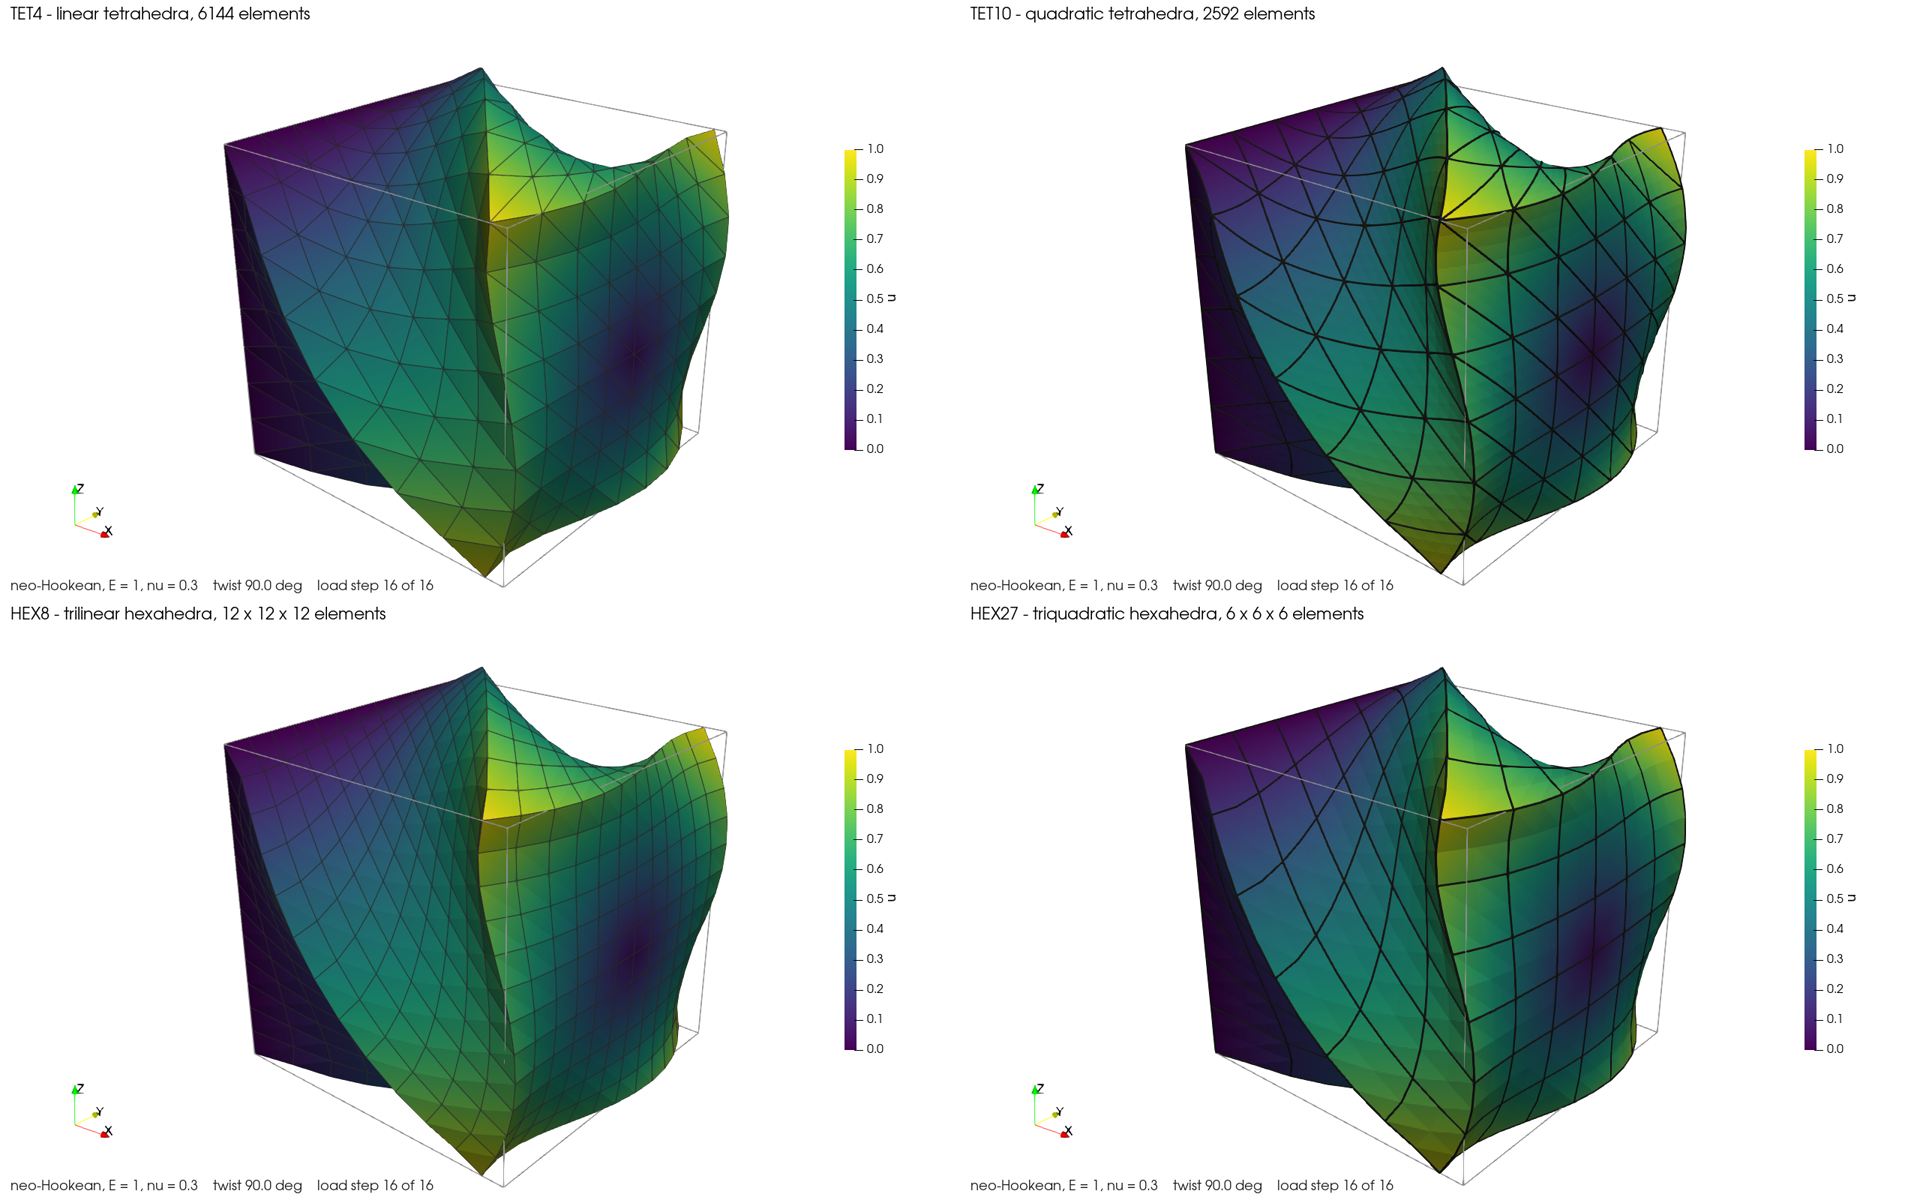
\includegraphics[width=\textwidth]{figures/twist_states.png}
\caption{The twist case at full load on coarse meshes of each element, coloured by the displacement
magnitude; the grey box is the undeformed cube.  Element edges of the quadratic elements are drawn
along their curved shape.  The Newton study runs the same case at about $10^6$~dof.}
\label{fig:twiststates}
\end{figure}

%% ===================================================================================================
\section{Results}
\label{sec:results}

\subsection{Correctness}

With an uncompressed double-precision store the application reproduces the exact matrix-free
application to round-off (\corrQpSixtyFourHexEight{} relative on HEX8, \corrQpSixtyFourTetFour{} on
TET4).  On TET10 the residual, the matrix-free and the BSR operators integrate with the $11$-point
rule, and the $P_2$-moment store agrees with BSR to \corrQpSixtyFourTetTen{}, on HEX27 the point store
to \corrQpSixtyFourHexTwentySeven{}: the rounding of the single-precision geometry, which grows as
the mesh is refined;
an $11$-point store of point values gives the same difference to every digit, which confirms that
the ten moments carry everything the quadrature sees.  In the Newton study the double-precision
store reproduces the exact operators' Newton and Krylov iteration counts on all four elements, and
the element matrices built from the store do the same.

\subsection{Application throughput, memory and set-up}

\begin{figure}[t]
\centering
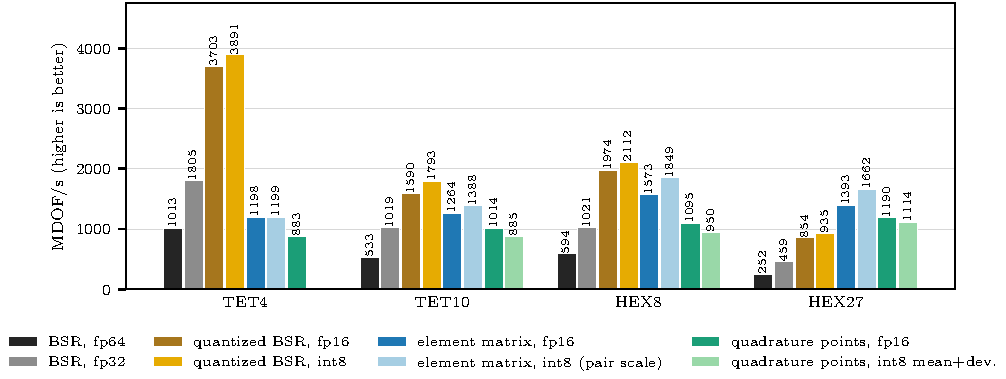
\includegraphics[width=\textwidth]{figures/throughput.pdf}
\caption{Application throughput against BSR, \benchdofHexEight{}~dof, Grace, $72$ threads.  The
element operators (matrix-free, projected, compressed stores, element matrices) use the packed
two-pass scatter; BSR is a row-parallel block product, the quantized matrix the product of
Section~\ref{sec:qbsr} (\texttt{int8} with a scale per block, \texttt{fp16} with one scale).  Missing bars: the mean-and-deviation
encodings need more than one stored tensor per element, which TET4 does not have.}
\label{fig:throughput}
\end{figure}

\begin{figure}[t]
\centering
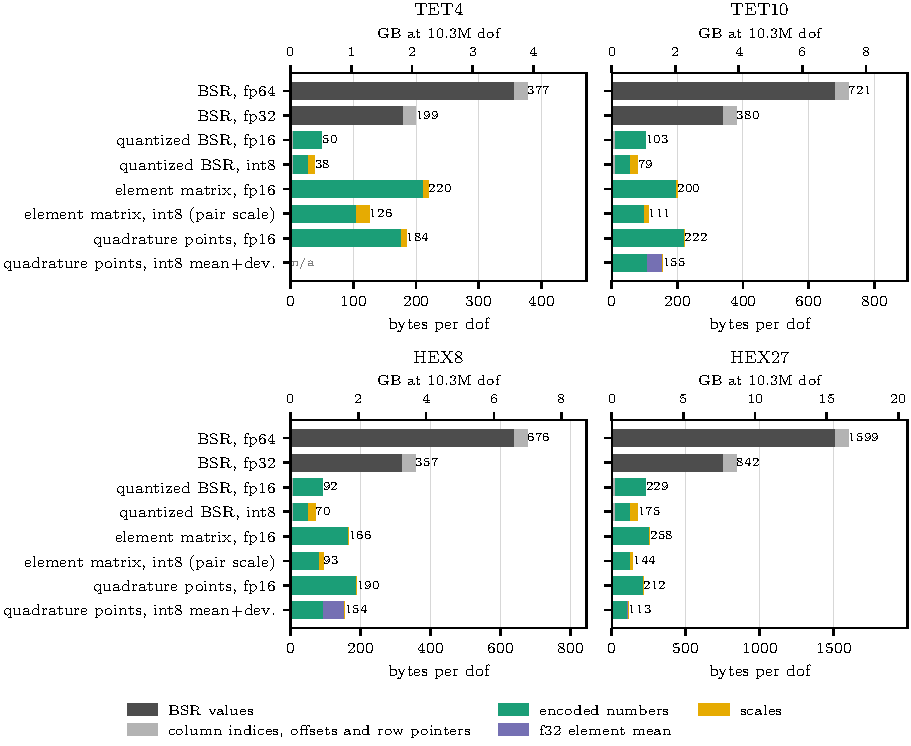
\includegraphics[width=\textwidth]{figures/memory_footprint.pdf}
\caption{Memory of the operator: BSR in double and single precision against the compressed
quadrature-point (or moment) store, the compressed element matrix and the quantized matrix.  Bars are the measured bytes
per degree of freedom (top axis: gigabytes at \benchdofHexEight{}~dof), split into the encoded
numbers and what accompanies them --- BSR's column indices and row pointers, the stores' scales and
the single-precision element mean of the mean-and-deviation encodings, the quantized matrix's scales
and column offsets (with its remainder).}
\label{fig:memory}
\end{figure}

Figures~\ref{fig:throughput} and~\ref{fig:memory} are the central comparison.  BSR is at the bandwidth bound the cost
model predicts ($\bsrSixtyFourRateHexEight$ and $\bsrThirtyTwoRateHexEight$~MDOF/s on HEX8 in
double and single precision).  On HEX8 and TET10 the half-precision store applies at
$\QpHalfVsThirtyTwoHexEight\times$ and $\QpHalfVsThirtyTwoTetTen\times$ the speed of single-precision
BSR and $\QpHalfVsSixtyFourHexEight\times$ and $\QpHalfVsSixtyFourTetTen\times$ that of double-precision
BSR, from $\QpHalfMemVsThirtyTwoHexEight$--$\QpHalfMemVsThirtyTwoTetTen\times$ less memory than the
former and $\QpHalfMemVsSixtyFourHexEight$--$\QpHalfMemVsSixtyFourTetTen\times$ less than the latter.
The \texttt{int8} mean-and-deviation store trades a further $\QpEightMdMemVsThirtyTwoHexEight$--%
$\QpEightMdMemVsThirtyTwoTetTen\times$ memory reduction against single-precision BSR for
$\QpEightMdVsThirtyTwoHexEight$ and $\QpEightMdVsThirtyTwoTetTen$ of its speed.  On HEX27, with
$\blocksHexTwentySeven$ blocks per matrix row, BSR is at its slowest
($\bsrThirtyTwoRateHexTwentySeven$~MDOF/s in single precision) and the half-precision store applies at
$\QpHalfVsThirtyTwoHexTwentySeven\times$ its speed from $\QpHalfMemVsThirtyTwoHexTwentySeven\times$ less
memory.  On TET4 BSR in single
precision stays ahead (the half-precision store applies at $\QpHalfVsThirtyTwoTetFour\times$ its
speed): with two elements per degree of freedom and fifteen blocks per matrix row, the matrix is
small and the element loop is not.

\begin{figure}[t]
\centering
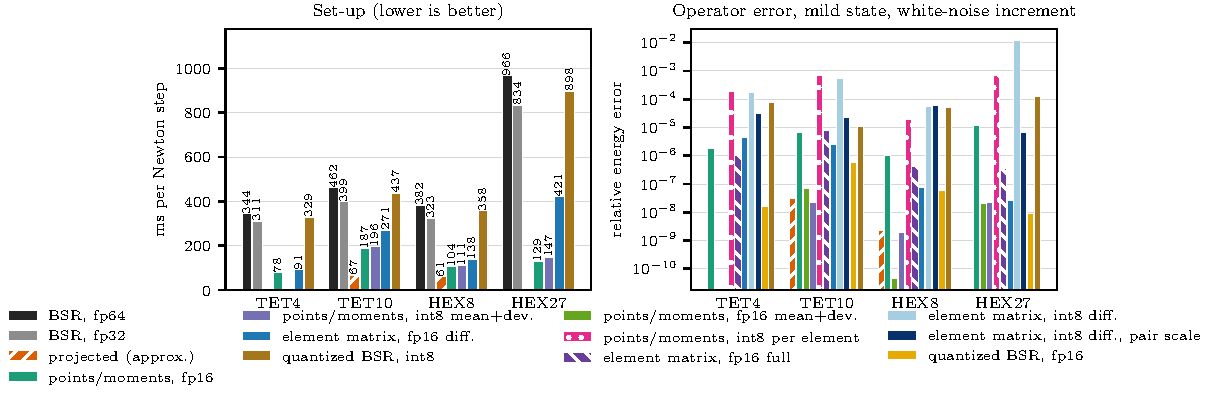
\includegraphics[width=\textwidth]{figures/setup_error.pdf}
\caption{Left: set-up of the operator once per Newton step, \benchdofHexEight{}~dof.  Right:
relative error in the energy of the operator against the exact one, at the mild state of the
application study, white-noise increment.}
\label{fig:setup}
\end{figure}

The set-up (Figure~\ref{fig:setup}, left) is where the compressed store gains most: evaluating and
encoding the point tangents costs a fraction of assembling the matrix, because it is the matrix
assembly without the element-matrix contraction and without the scatter into the sparse pattern.

\subsection{Accuracy and the Newton iteration}

\begin{figure}[t]
\centering
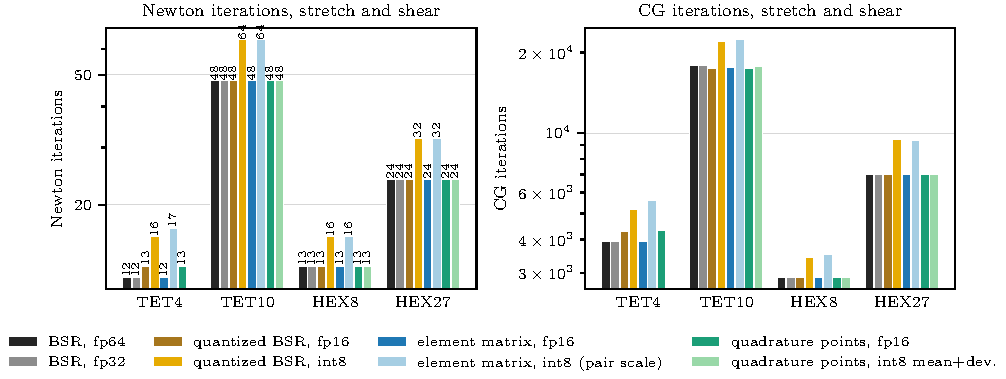
\includegraphics[width=\textwidth]{figures/newton_iterations.pdf}
\caption{Newton and conjugate-gradient iterations to solution, about $1.08\times10^6$~dof, four
load steps (TET10: sixteen).  BSR in both precisions, the matrix-free operator and the
double-precision store have identical counts, shown once.}
\label{fig:newton}
\end{figure}

The error of the encodings in a white-noise energy measure (Figure~\ref{fig:setup}, right) does
not predict their effect on the iteration; the iteration counts (Figure~\ref{fig:newton}) do, and
they follow Section~\ref{sec:errormodel}.  The projected operator costs
$\newtonPzeroExtraHexEight\%$ more Newton iterations on HEX8 and $\newtonPzeroExtraTetTen\%$ more on
TET10, and nothing on TET4, where it is exact.  \texttt{int8} with one scale per element, whose
absolute error is set by the largest entry of the tangent, is not usable as a Newton operator.  The
half-precision and both mean-and-deviation stores keep the exact iteration counts on HEX8 and
TET10.
\IfFileExists{figures/newton_twist.pdf}{%
Under large deformation (a $90^\circ$ twist, Figure~\ref{fig:twist}) the same ordering holds,
and the element matrices separate by form: in half precision the difference form keeps the exact
count while the full matrix, whose rounding does not preserve the rigid translations, costs
iterations, and \texttt{int8} costs iterations in either form.

\begin{figure}[t]
\centering
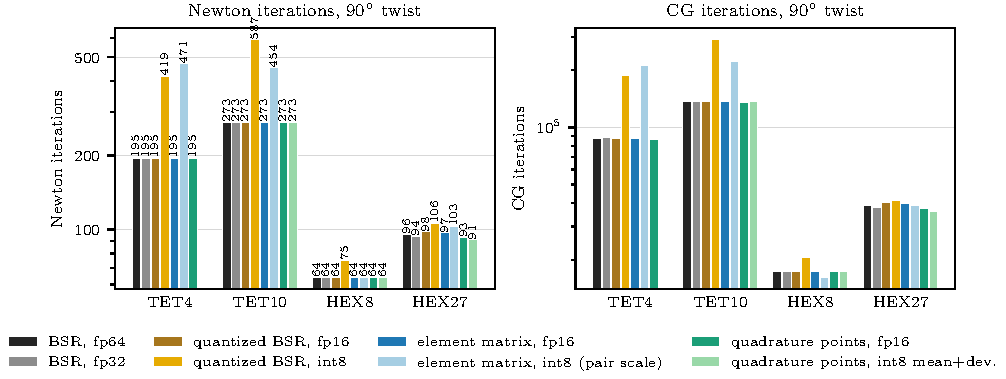
\includegraphics[width=\textwidth]{figures/newton_twist.pdf}
\caption{Newton and conjugate-gradient iterations for a $90^\circ$ twist of the cube in sixteen load
steps.}
\label{fig:twist}
\end{figure}}{}

\subsection{Time to solution and problem size}

\begin{figure}[t]
\centering
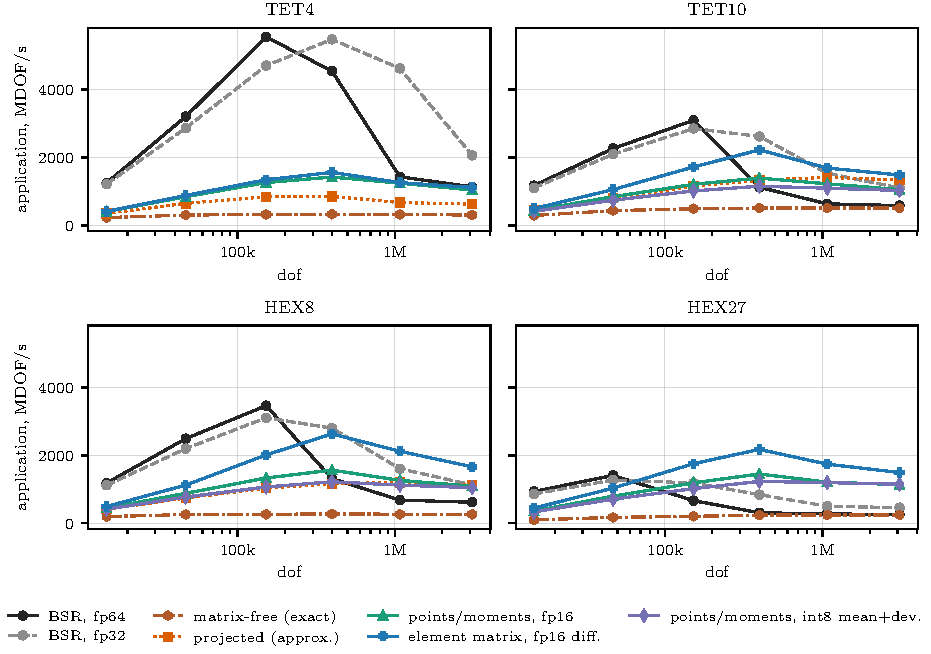
\includegraphics[width=\textwidth]{figures/sweep_throughput.pdf}\\[1ex]
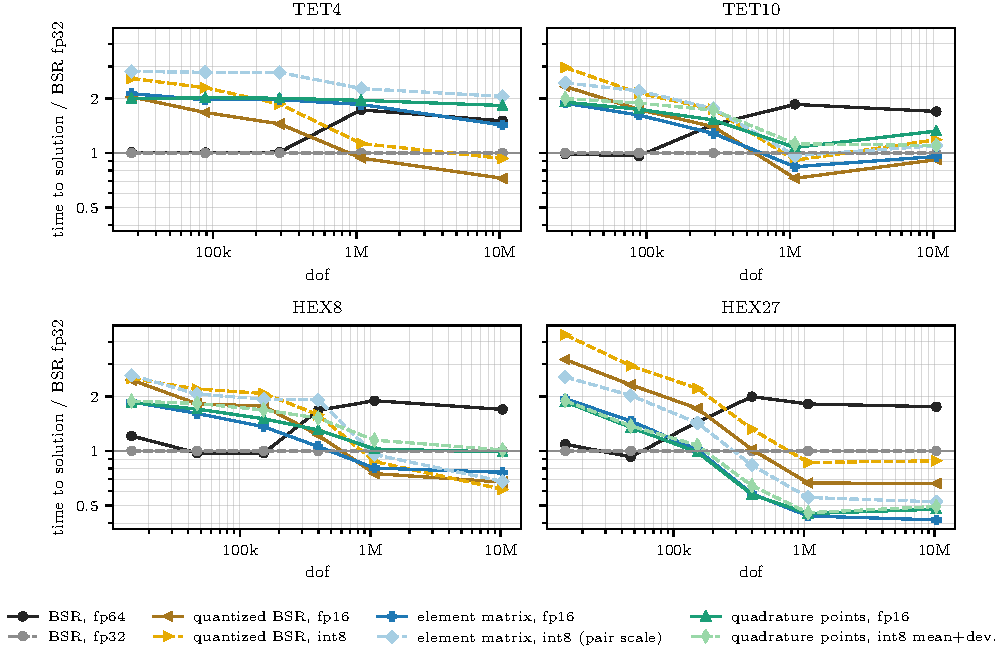
\includegraphics[width=\textwidth]{figures/sweep_newton.pdf}
\caption{Against problem size, Grace, $72$ threads.  Top: application throughput.  Bottom: Newton
time to solution relative to BSR in single precision (below one is faster).  The largest points of
the bottom row are the saturated runs of Figure~\ref{fig:tts}.}
\label{fig:sweep}
\end{figure}

The comparison depends on the problem size, and Figure~\ref{fig:sweep} shows how.  While the
matrix fits in the last-level cache --- up to about half a million degrees of freedom for the
elements here --- the BSR product runs at two to three times its bandwidth bound, and no element
operator comes close: the compressed stores are compute-bound at every size, and their throughput
only saturates once every thread has enough packs.  The penalty is therefore at small problem
sizes, and the regime in which the compressed store competes is the one the cost model was written
for, where the sparse matrix streams from memory.  At about $10^7$ degrees of freedom on HEX8
(Figure~\ref{fig:tts}) the half-precision store solves in $\timeQpHalfHexEight\times$ and the
\texttt{int8} mean-and-deviation store in $\timeQpEightMdHexEight\times$ the time of
single-precision BSR, against $\timeBsrSixtyFourHexEight\times$ for double-precision BSR, with
$\QpHalfMemVsThirtyTwoHexEight\times$ and $\QpEightMdMemVsThirtyTwoHexEight\times$ less operator
memory than single-precision BSR.  On HEX27 the two stores take $\timeQpHalfHexTwentySeven\times$ and
$\timeQpEightMdHexTwentySeven\times$ its time; on TET10, where they apply at about its speed,
$\timeQpHalfTetTen\times$ and $\timeQpEightMdTetTen\times$, the half-precision store with more Newton
iterations at this size.  The half-precision element matrix in difference form takes
$\timeEaDiffHalfHexEight\times$, $\timeEaDiffHalfTetTen\times$ and $\timeEaDiffHalfHexTwentySeven\times$
the time of single-precision BSR on HEX8, TET10 and HEX27.  On TET4 every run at this size meets a
load step that diverges, and the number of iterations each operator spends before the divergence is
detected decides the comparison there.

\begin{figure}[t]
\centering
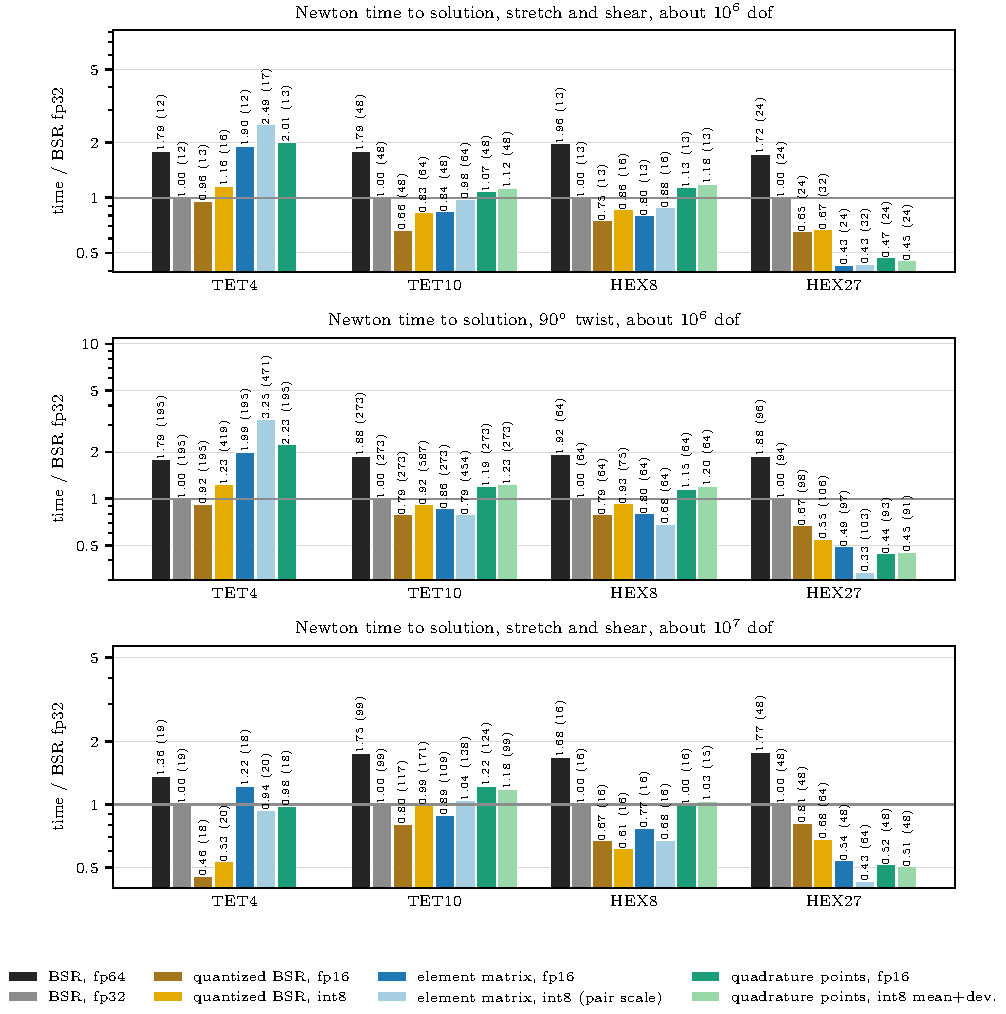
\includegraphics[width=\textwidth]{figures/time_to_solution.pdf}
\caption{Newton time to solution relative to BSR in single precision (log scale, below one is
faster): the stretch case at about $10^6$ and $10^7$~dof and the twist at about $10^6$~dof.  Each
bar is labelled with the ratio and, in parentheses, the Newton iterations of the run; a count that
differs from BSR's marks a run that took a different load-step path.  Failed load-step attempts
are not counted in the iterations but are included in the time.}
\label{fig:tts}
\end{figure}

\subsection{Element matrices}

The element matrices of Section~\ref{sec:elementmatrix} are built by the same set-up kernel and
applied through the same scatter, and they are the fastest element operators measured
(Figure~\ref{fig:throughput}).  In half precision and difference form they apply at
$\EaDiffHalfRateHexEight$ and $\EaDiffHalfRateTetTen$~MDOF/s on HEX8 and TET10,
$\EaDiffHalfVsThirtyTwoHexEight\times$ and $\EaDiffHalfVsThirtyTwoTetTen\times$ the speed of
single-precision BSR from $\EaDiffHalfMemVsThirtyTwoHexEight\times$ and
$\EaDiffHalfMemVsThirtyTwoTetTen\times$ less memory (Figure~\ref{fig:memory}); in \texttt{int8} the
factors grow to $\EaDiffEightVsThirtyTwoHexEight\times$ and $\EaDiffEightVsThirtyTwoTetTen\times$ in
speed.  The difference form is faster than the full matrix and, as designed, more accurate under
the same encoding (Figure~\ref{fig:setup}, right); in the Newton study its half-precision encoding
keeps the exact iteration counts where the full matrix in half precision does not
(Figure~\ref{fig:twist}).  Their set-up contracts the stored tensors per element, vectorised over the lanes of a
block of elements and computing only the blocks above the diagonal ($\SetupEaDiffHalfHexEight$~ms on
HEX8 against $\SetupQpHalfHexEight$ for the half-precision point store and
$\SetupBsrThirtyTwoHexEight$ for single-precision BSR assembly; $\SetupEaDiffHalfTetTen$,
$\SetupQpHalfTetTen$ and $\SetupBsrThirtyTwoTetTen$ on TET10): the contraction is where the element
matrix pays for its smaller application.  On TET4 the double-precision element matrices were
measured at $3.1\times10^6$~dof only; their bytes per degree of freedom enter
Figure~\ref{fig:memory}.

On HEX27 the element matrix is the larger store (Table~\ref{tab:elementmatrix}) and still the faster
operator: in half precision and difference form it applies at
$\EaDiffHalfVsThirtyTwoHexTwentySeven\times$ the speed of single-precision BSR, against
$\QpHalfVsThirtyTwoHexTwentySeven\times$ for the half-precision point store.  With one scale per element
\texttt{int8} spends its range on the largest node-pair block there: its energy error is
\errEaDiffEightHexTwentySeven{}, against \errEaPairEightHexTwentySeven{} with a scale per node pair
\eqref{eq:pairscale}, which costs $\pairSlowdownHexTwentySeven\%$ of the throughput.  On TET10 and
TET4 the pair scale divides the error by $\pairErrGainTetTen$ and $\pairErrGainTetFour$; on HEX8, whose
node pairs are of similar size, it gains nothing and costs $\pairSlowdownHexEight\%$.  The Newton
iteration shows the difference: at about $10^6$~dof the element-scaled \texttt{int8} matrix needs
$\newtonEaDiffEightHexTwentySeven$ Newton iterations on HEX27 and $\newtonEaDiffEightTetTen$ on TET10,
against $\newtonExactHexTwentySeven$ and $\newtonExactTetTen$ for the exact operators, the
pair-scaled one $\newtonEaPairEightHexTwentySeven$ and $\newtonEaPairEightTetTen$, and the
half-precision difference form keeps the exact counts.  Under the twist the pair scale restores the
exact count on HEX8 ($\twistEaPairEightHexEight$ against $\twistEaDiffEightHexEight$ with one scale per
element) and nearly on HEX27 ($\twistEaPairEightHexTwentySeven$ against $\twistEaDiffEightHexTwentySeven$,
exact $\twistExactHexTwentySeven$), but not on TET4, where both \texttt{int8} matrices more than double
the exact $\twistExactTetFour$ iterations ($\twistEaDiffEightTetFour$ and $\twistEaPairEightTetFour$)
although the pair scale divides TET4's white-noise error by $\pairErrGainTetFour$ --- another
instance of that measure not predicting the iteration --- and the half-precision matrix remains the
choice there.

\subsection{Quantized assembled matrices}

The quantized matrix of Section~\ref{sec:qbsr} is the fastest operator on three of the four
elements (Figure~\ref{fig:throughput}).  In \texttt{int8} it applies at $\QbsrEightVsThirtyTwoTetFour$,
$\QbsrEightVsThirtyTwoTetTen$, $\QbsrEightVsThirtyTwoHexEight$ and $\QbsrEightVsThirtyTwoHexTwentySeven\times$
the speed of single-precision BSR on TET4, TET10, HEX8 and HEX27, from
$\QbsrEightMemVsThirtyTwoTetTen$--$\QbsrEightMemVsThirtyTwoTetFour\times$ less memory
(Figure~\ref{fig:memory}), and in \texttt{fp16} at $\QbsrHalfVsThirtyTwoTetTen$--$\QbsrHalfVsThirtyTwoTetFour\times$.
Storing each pair once makes it $\upperGainHexTwentySeven$--$\upperGainHexEight\times$ faster than the
full difference form from $\upperMemTetTen$--$\upperMemTetFour\times$ less memory, and the column offsets
save a further $\offsetSavingHexEight\%$.  The product is not bandwidth-bound: it moves
$\gbsQbsrEightHexEight$~GB/s on HEX8 against $\gbsBsrThirtyTwoHexEight$ for single-precision BSR, since
every stored block reads its own $h_j$, which an element operator reads once per element node.  On
HEX27, whose rows have the most blocks, the element matrix with a scale per node pair stays ahead
($\EaPairEightRateHexTwentySeven$ against $\QbsrEightRateHexTwentySeven$~MDOF/s).  Its set-up is BSR's
assembly plus the encoding ($\SetupQbsrEightHexEight$ against $\SetupBsrThirtyTwoHexEight$~ms on HEX8).

In the Newton study the \texttt{fp16} matrix keeps the iteration counts of BSR at about $10^6$
degrees of freedom ($\newtonQbsrHalfHexEight$, $\newtonQbsrHalfTetTen$ and $\newtonQbsrHalfHexTwentySeven$
on HEX8, TET10 and HEX27, one more on TET4) and under the twist (on HEX27 $\twistQbsrHalfHexTwentySeven$
against $\twistExactHexTwentySeven$); at about $10^7$ on TET10 it needs
$\tenmNewtonQbsrHalfTetTen$ against $\tenmNewtonExactTetTen$, as the half-precision point store does.
\texttt{int8} with a scale per block needs about a third more ($\newtonQbsrEightTetTen$ against
$\newtonExactTetTen$ on TET10 at $10^6$), as the element matrix with a scale per node pair.  At about
$10^7$ degrees of freedom the \texttt{fp16} matrix solves in $\timeQbsrHalfTetFour$, $\timeQbsrHalfTetTen$,
$\timeQbsrHalfHexEight$ and $\timeQbsrHalfHexTwentySeven\times$ the time of single-precision BSR on TET4,
TET10, HEX8 and HEX27, and the \texttt{int8} matrix in $\timeQbsrEightTetFour$, $\timeQbsrEightTetTen$,
$\timeQbsrEightHexEight$ and $\timeQbsrEightHexTwentySeven\times$ (Figure~\ref{fig:tts}): the fastest
operator measured on the tetrahedra, level with the element matrices on HEX8
($\timeEaPairEightHexEight\times$ with a scale per node pair), and behind them on HEX27
($\timeEaPairEightHexTwentySeven\times$).

The application reads $\storeQbsrEightHexEight$~GiB on HEX8 at $\peakDofHexEight$ degrees of freedom,
but the peak memory of the whole Newton run is $\peakQbsrEightHexEight$~GiB, against
$\peakBsrThirtyTwoHexEight$ for single-precision BSR and $\peakEaPairEightHexEight$ for the \texttt{int8}
element matrix with a scale per node pair (on TET4: $\peakQbsrEightTetFour$, $\peakBsrThirtyTwoTetFour$
and $\peakEaPairEightTetFour$~GiB).  The single-precision assembly and the node graph it is built on set
the peak, not the store; assembling and encoding the matrix in chunks of rows would remove the first.

%% ===================================================================================================
\section{Discussion and limitations}
\label{sec:discussion}

\paragraph{Where the compressed operators pay.}  Their advantage is bandwidth, so it appears
where the sparse matrix streams from memory (Figure~\ref{fig:sweep}).  In Newton time to solution
on one Grace CPU the compressed operators beat single-precision BSR on HEX27, whose matrix has the
most blocks per row, from a few $10^5$ degrees of freedom; on HEX8 and TET10 the half-precision
element matrix does from about $10^6$, while the point stores draw level with single-precision BSR
on HEX8 at $10^7$ and stay behind it on TET10.  Below that the matrix lives in cache and BSR is
two to three times faster than its bandwidth bound; no element operator, compressed or not,
competes there.  In a distributed run this is a statement about the problem size per node.  The
set-up, where the compressed stores are cheapest, is a small part of a Newton step at the Krylov
tolerances used here; it matters more when the Krylov iteration is short.

\paragraph{The quantized matrix.}  Quantizing BSR itself, in difference form with each pair of blocks
stored once, is the strongest competitor of the element operators at $10^7$ degrees of freedom: it is
the fastest operator measured on linear and quadratic tetrahedra, where a matrix row has few blocks
and the element operators repeat each coupling in every element that shares it, and level with the
element matrices on trilinear hexahedra.  The element matrices keep the advantage where the matrix
rows are long (HEX27), since they gather each node once per element, and in peak memory, since they
need neither a single-precision assembly nor the node graph.

\paragraph{Points or element matrices.}  At the orders studied the element matrix is no larger than
the minimal point store on HEX8 and TET10 and cheaper to apply, so it is the better compressed
object there, provided its set-up is as efficient as the point store's.  The point store wins on
TET4, whose single point is smaller than its matrix, and wherever the element matrix grows faster
than the quadrature --- with polynomial degree, since the matrix grows as the square of the node
count.  HEX27 is past the crossover in memory but not in operations: its element matrix is a tenth
larger than the point store and still needs fewer operations than the sum-factorised point schedule,
and it is the faster operator measured on it.

\paragraph{What the error measure must see.}  A relative error per stored number, or an operator
error measured against white noise, does not predict the effect on Newton's method; the iteration
counts do.  The modes that decide it are smooth and locally nearly rigid, where the element operator
is close to singular: an encoding whose absolute error there is set by the largest entry of the
tangent costs iterations, one whose error is set by the variation of the tangent over the element,
or which keeps the rigid translations exact, does not.

\paragraph{Limitations.}  The study uses one material, structured meshes, and a Krylov method
without preconditioner, chosen so that every operator runs the same iteration; with a
preconditioner built from the operator, the encodings change the preconditioner too.  Materials
defined by a residual carry $81$ numbers per point.  The packed traversal is sensitive to the number
of packs per thread, which the library's default pack size leaves too low below about $10^6$
degrees of freedom on 72 threads; the measurements set it for every operator alike.

%% ===================================================================================================
\section{Conclusions}

Storing the pulled-back tangent at the quadrature points --- or, on quadratic tetrahedra, its $P_2$
moments, which is all the quadrature sees --- removes the approximation of the element-constant
projection and the Newton iterations it costs, and compressing what is stored brings the operator
below the memory of a single-precision sparse matrix.  Half precision, or \texttt{int8} deviations
from the element mean, keep the exact iteration counts; \texttt{int8} with one scale per element does
not.  Built from the same stored tensors, quantized element matrices in difference form are faster
still and keep rigid translations exactly.  On one Grace CPU at $10^7$ degrees of freedom the
compressed operators apply at or above the speed of single-precision BSR on hexahedra and quadratic
tetrahedra, from up to a quarter of double-precision BSR's memory, and the half-precision element matrix
solves the Newton problems faster than single-precision BSR on all three; BSR remains the better
choice for linear tetrahedra and for problems small enough to keep the matrix in cache.  The same
encodings applied to the assembled matrix, in difference form with each pair of blocks stored once,
make the matrix itself the fastest operator on linear and quadratic tetrahedra and match the element
matrices on trilinear hexahedra, at the peak memory of its single-precision assembly; on triquadratic
hexahedra the element matrices remain ahead.

\begin{thebibliography}{99}

\bibitem{Abdelfattah2021}
A.~Abdelfattah et al.
\newblock A survey of numerical linear algebra methods utilizing mixed-precision arithmetic.
\newblock \emph{Int. J. High Perform. Comput. Appl.}, 35(4):344--369, 2021.

\bibitem{Ahmad2019}
K.~Ahmad, H.~Sundar, M.~Hall.
\newblock Data-driven mixed precision sparse matrix vector multiplication for GPUs.
\newblock \emph{ACM Trans. Archit. Code Optim.}, 16(4), 2019.

\bibitem{Alappat2020}
C.~Alappat, G.~Hager, O.~Schenk, J.~Thies, A.~Basermann, A.~R. Bishop, H.~Fehske, G.~Wellein.
\newblock A recursive algebraic coloring technique for hardware-efficient symmetric sparse
matrix--vector multiplication.
\newblock \emph{ACM Trans. Parallel Comput.}, 7(3):19, 2020.

\bibitem{MFEM2021}
R.~Anderson et al.
\newblock MFEM: A modular finite element methods library.
\newblock \emph{Comput. Math. Appl.}, 81:42--74, 2021.

\bibitem{Anzt2019}
H.~Anzt, J.~Dongarra, G.~Flegar, N.~J. Higham, E.~S. Quintana-Ort\'{\i}.
\newblock Adaptive precision in block-Jacobi preconditioning for iterative sparse linear system solvers.
\newblock \emph{Concurrency Computat. Pract. Exper.}, 31(6):e4460, 2019.

\bibitem{BonetWood2008}
J.~Bonet, R.~D. Wood.
\newblock \emph{Nonlinear Continuum Mechanics for Finite Element Analysis}.
\newblock Cambridge University Press, 2nd edition, 2008.

\bibitem{libCEED2021}
J.~Brown et al.
\newblock libCEED: Fast algebra for high-order element-based discretizations.
\newblock \emph{J. Open Source Softw.}, 6(63):2945, 2021.

\bibitem{Brown2022}
J.~Brown et al.
\newblock Performance portable solid mechanics via matrix-free $p$-multigrid.
\newblock arXiv:2204.01722, 2022.

\bibitem{Davydov2020}
D.~Davydov, J.-P. Pelteret, D.~Arndt, M.~Kronbichler, P.~Steinmann.
\newblock A matrix-free approach for finite-strain hyperelastic problems using geometric multigrid.
\newblock \emph{Int. J. Numer. Methods Eng.}, 121(13):2874--2895, 2020.

\bibitem{DemboEisenstatSteihaug1982}
R.~S. Dembo, S.~C. Eisenstat, T.~Steihaug.
\newblock Inexact Newton methods.
\newblock \emph{SIAM J. Numer. Anal.}, 19(2):400--408, 1982.

\bibitem{DevilleFischerMund2002}
M.~O. Deville, P.~F. Fischer, E.~H. Mund.
\newblock \emph{High-Order Methods for Incompressible Fluid Flow}.
\newblock Cambridge University Press, 2002.

\bibitem{EisenstatWalker1996}
S.~C. Eisenstat, H.~F. Walker.
\newblock Choosing the forcing terms in an inexact Newton method.
\newblock \emph{SIAM J. Sci. Comput.}, 17(1):16--32, 1996.

\bibitem{Elafrou2019}
A.~Elafrou, G.~Goumas, N.~Koziris.
\newblock Conflict-free symmetric sparse matrix-vector multiplication on multicore architectures.
\newblock In \emph{Proc. Int. Conf. High Performance Computing, Networking, Storage and Analysis
(SC'19)}, ACM, 2019.

\bibitem{Gruetzmacher2023}
T.~Gr\"utzmacher, H.~Anzt, E.~S. Quintana-Ort\'{\i}.
\newblock Using Ginkgo's memory accessor for improving the accuracy of memory-bound low precision BLAS.
\newblock \emph{Softw. Pract. Exper.}, 53(1):81--98, 2023.

\bibitem{HighamMary2022}
N.~J. Higham, T.~Mary.
\newblock Mixed precision algorithms in numerical linear algebra.
\newblock \emph{Acta Numerica}, 31:347--414, 2022.

\bibitem{Keast1986}
P.~Keast.
\newblock Moderate-degree tetrahedral quadrature formulas.
\newblock \emph{Comput. Methods Appl. Mech. Engrg.}, 55(3):339--348, 1986.

\bibitem{Kelley2018}
C.~T. Kelley.
\newblock Numerical methods for nonlinear equations.
\newblock \emph{Acta Numerica}, 27:207--287, 2018.

\bibitem{KronbichlerKormann2012}
M.~Kronbichler, K.~Kormann.
\newblock A generic interface for parallel cell-based finite element operator application.
\newblock \emph{Comput. Fluids}, 63:135--147, 2012.

\bibitem{KronbichlerKormann2019}
M.~Kronbichler, K.~Kormann.
\newblock Fast matrix-free evaluation of discontinuous Galerkin finite element operators.
\newblock \emph{ACM Trans. Math. Softw.}, 45(3):29, 2019.

\bibitem{KronbichlerLjungkvist2019}
M.~Kronbichler, K.~Ljungkvist.
\newblock Multigrid for matrix-free high-order finite element computations on graphics processors.
\newblock \emph{ACM Trans. Parallel Comput.}, 6(1):2, 2019.

\bibitem{Kreutzer2014}
M.~Kreutzer, G.~Hager, G.~Wellein, H.~Fehske, A.~R. Bishop.
\newblock A unified sparse matrix data format for efficient general sparse matrix-vector multiplication
on modern processors with wide SIMD units.
\newblock \emph{SIAM J. Sci. Comput.}, 36(5):C401--C423, 2014.

\bibitem{Lindstrom2014}
P.~Lindstrom.
\newblock Fixed-rate compressed floating-point arrays.
\newblock \emph{IEEE Trans. Vis. Comput. Graph.}, 20(12):2674--2683, 2014.

\bibitem{Orszag1980}
S.~A. Orszag.
\newblock Spectral methods for problems in complex geometries.
\newblock \emph{J. Comput. Phys.}, 37(1):70--92, 1980.

\bibitem{Rouhani2023}
B.~D. Rouhani, R.~Zhao, A.~More, et al.
\newblock Microscaling data formats for deep learning.
\newblock arXiv:2310.10537, 2023.

\bibitem{Schussnig2025}
R.~Schussnig, N.~Fehn, P.~Munch, M.~Kronbichler.
\newblock Matrix-free higher-order finite element methods for hyperelasticity.
\newblock \emph{Comput. Methods Appl. Mech. Engrg.}, 435:117600, 2025.

\bibitem{Tezcan2022}
E.~Tezcan, T.~Torun, F.~Ko\c{s}ar, K.~Kaya, D.~Unat.
\newblock Mixed and multi-precision SpMV for GPUs with row-wise precision selection.
\newblock In \emph{Proc. 34th Int. Symp. Computer Architecture and High Performance Computing
(SBAC-PAD)}, IEEE, 2022.

\bibitem{Wichrowski2025}
M.~Wichrowski, M.~Rezaee-Hajidehi, J.~Korelc, M.~Kronbichler, S.~Stupkiewicz.
\newblock Matrix-free methods for finite-strain elasticity: automatic code generation with no
performance overhead.
\newblock arXiv:2505.15535, 2025.

\bibitem{ZulianPA}
P.~Zulian.
\newblock Partial assembly by $L^2$-projection: node-level performance of generated inexact
tangent kernels for finite-strain elasticity.
\newblock In preparation.

\end{thebibliography}

\end{document}
